
\documentclass[a4paper,8pt]{extarticle} % extarticle allows to use font size of 8pt.

\usepackage[a4paper, top=1.6cm, bottom=2cm, left=1.6cm, right=1.6cm]{geometry} % Marge reduction.

\usepackage{ifxetex}

\ifxetex
  \usepackage{fontspec}
  \defaultfontfeatures{Ligatures=TeX} % To support LaTeX quoting style
  \setmainfont{Casablanca Antique}
\else
	\usepackage[T1]{fontenc} 		% Font encoding.
	\usepackage[utf8]{inputenc} 	% Document encoding.
	\usepackage{palatino} 			% Font.
\fi

\usepackage{microtype}			% Greatly improves general appearance of the text.
\usepackage{SIunits}			% Unit appearance.
\usepackage{array}				% Additionnal options for arrays.
\usepackage{colortbl}			% Additionnal options for coloring arrays.
\usepackage{multicol}			% Allows to divide a part of the page in multiple columns.
\usepackage{framed}				% Boxes.
\usepackage[inline]{enumitem}   % Display inline lists.
\usepackage{etoolbox}           % General utility. Good for lists for instance.
\usepackage{newfloat}			% Used to create new flottable environnements.
	\DeclareFloatingEnvironment[placement=htbp!]{unitframeFlot}
\usepackage{keyval}             % Used to create maps of commands/labels/objects.
	\makeatletter                  % Mandatory for the usage of keyval.
\usepackage{xstring}            % String parsing, cutting, etc.
\usepackage{xparse}             % List utilities.
\usepackage{xspace}				% Define commands that appear not to eat spaces.
\usepackage{textcomp} 			% for the straight single quote \textquotesingle.
\usepackage[colorlinks=true]{hyperref} % Links in PDF.
\usepackage[framemethod=TikZ]{mdframed}% For fancy frames.
\usepackage{tikz}				% For fancy frames.

%%% Language specific stuff

% \usepackage[french]{babel}

\frenchbsetup{StandardLists=true} % Necessary to use enumitem with babel/french.

% This has to disappear.

\newcommand{\pouce}{\inch}
\newcommand{\pied}{\foot}
\newcommand{\portee}{\range}

% Labels

\newcommand{\labels@range}{Portée}
\newcommand{\labels@profile}{Profil}
\newcommand{\labels@M}{M}
\newcommand{\labels@WS}{CC}
\newcommand{\labels@BS}{CT}
\newcommand{\labels@S}{F}
\newcommand{\labels@T}{E}
\newcommand{\labels@W}{PV}
\newcommand{\labels@I}{I}
\newcommand{\labels@A}{A}
\newcommand{\labels@Ld}{Cd}
\newcommand{\labels@unitsize}{Taille de l'unité}
\newcommand{\labels@basesize}{Taille du socle}
\newcommand{\labels@trooptype}{Type de troupe}
\newcommand{\labels@specialrules}{Règles spéciales}
\newcommand{\labels@equipment}{Équipement}
\newcommand{\labels@options}{Options}
\newcommand{\labels@commandgroup}{État-Major}
\newcommand{\labels@lords}{Seigneurs}
\newcommand{\labels@heroes}{Héros}
\newcommand{\labels@baseunits}{Unités de base}
\newcommand{\labels@specialunits}{Unités spéciales}
\newcommand{\labels@rareunits}{Unités rares}
\newcommand{\labels@mounts}{Montures}
\newcommand{\labels@specialequipment}{Équipement spécial}
\newcommand{\labels@fantasybattles}{Batailles Fantastiques}
\newcommand{\labels@NinthAge}{Le 9\ieme Âge}
\newcommand{\labels@creators}{Une collaboration des créateurs de l'ETC et du Swedish Comp System}
\newcommand{\labels@latexcredit}{Document réalisé à l'aide de \LaTeX .}

\newcommand{\labels@point}{pt}
\newcommand{\labels@points}{pts}

\newcommand{\labels@armyspecialrules}{Règles spéciales de l'armée}
\newcommand{\labels@armoury}{Armurerie}
\newcommand{\labels@magicitems}{Objets magiques}

% Technical

\newcommand{\free}{gratuit}
\newcommand{\upto}{jusqu'à}
\newcommand{\unlimited}{sans limite de pts}
\newcommand{\permodel}{/fig.}

% Special rules

\newcommand{\ambush}{\specialrule{Embuscade}\xspace}
\newcommand{\armourpiercing}[1]{\specialrule{Perforant\ifblank{#1}{}{~(#1)}}\xspace}
\newcommand{\blurry}{\specialrule{Camouflé}\xspace}
\newcommand{\bodyguard}[1]{\specialrule{Garde du Corps\ifblank{#1}{}{~(#1)}}\xspace}
\newcommand{\breathweapon}[1]{\specialrule{Attaque de Souffle\ifblank{#1}{}{ (#1)}}\xspace}
\newcommand{\channel}{\specialrule{Canalisation}\xspace}
\newcommand{\crushattack}{\specialrule{Attaque Écrasante}\xspace}
\newcommand{\devastatingcharge}{\specialrule{Charge Dévastatrice}\xspace}
\newcommand{\distracting}{\specialrule{Distrayant}\xspace}
\newcommand{\engineer}{\specialrule{Ingénieur}\xspace}
\newcommand{\ethereal}{\specialrule{Éthéré}\xspace}
\newcommand{\fastcavalry}{\specialrule{Cavalerie Légère}\xspace}
\newcommand{\fear}{\specialrule{Peur}\xspace}
\newcommand{\fightinextrarank}{\specialrule{Combat avec un Rang Supplémentaire}\xspace}
\newcommand{\fireborn}{\specialrule{Né du Feu}\xspace}
\newcommand{\flamingattacks}{\specialrule{Attaques Enflammées}\xspace}
\newcommand{\flammable}{\specialrule{Inflammable}\xspace}
\newcommand{\freereform}{\specialrule{Reformation Gratuite}\xspace}
\newcommand{\frenzy}{\specialrule{Frénésie}\xspace}
\newcommand{\fly}[1]{\specialrule{Vol\ifblank{#1}{}{~(#1)}}\xspace}
\newcommand{\grindingattacks}[1]{\specialrule{Attaques de Broyage\ifblank{#1}{}{~(#1)}}\xspace}
\newcommand{\hatred}{\specialrule{Haine}\xspace}
\newcommand{\hellfire}{\specialrule{Flammes de l'Enfer}\xspace}
\newcommand{\hidden}{\specialrule{Caché}\xspace}
\newcommand{\holyattacks}{\specialrule{Attaques Sacrées}\xspace}
\newcommand{\immunetopsychology}{\specialrule{Immunisé à la Psychologie}\xspace}
\newcommand{\impacthits}[1]{\specialrule{Touches d'Impact\ifblank{#1}{}{~(#1)}}\xspace}
\newcommand{\insignificant}{\specialrule{Insignifiant}\xspace}
\newcommand{\largetarget}{\specialrule{Grande Cible}\xspace}
\newcommand{\lethalstrike}{\specialrule{Coup Fatal}\xspace}
\newcommand{\lightningattacks}{\specialrule{Attaques Foudroyantes}\xspace}
\newcommand{\lightningreflexes}{\specialrule{Réflexes Foudroyants}\xspace}
\newcommand{\magicresistance}[1]{\specialrule{Résistance à la Magie\ifblank{#1}{}{~(#1)}}\xspace}
\newcommand{\magicalattacks}{\specialrule{Attaques Magiques}\xspace}
\newcommand{\metalshifting}{\specialrule{Fusion du Métal}\xspace}
\newcommand{\moveorfire}{\specialrule{Mouvement ou Tir}\xspace}
\newcommand{\multipleshots}[1]{\specialrule{Tirs Multiples\ifblank{#1}{}{ (#1)}}\xspace}
\newcommand{\multiplewounds}[2]{\specialrule{Blessures Multi\-ples\ifblank{#1}{}{ (#1\ifblank{#2}{)}{, #2)}}\xspace}}
\newcommand{\notaleader}{\specialrule{Pas un Meneur}\xspace}
\newcommand{\otherworldly}{\specialrule{D'Outre-Monde}\xspace}
\newcommand{\pathmaster}[1]{\specialrule{Maître de la Discipline\ifblank{#1}{}{ (#1)}}\xspace}
\newcommand{\poisonedattacks}{\specialrule{Attaques Empoisonnées}\xspace}
\newcommand{\quicktofire}{\specialrule{Tir Rapide}\xspace}
\newcommand{\randommovement}[1]{\specialrule{Mouvement Aléatoire\ifblank{#1}{}{~(#1)}}\xspace}
\newcommand{\randomattacks}[1]{\specialrule{Attaques Aléatoires\ifblank{#1}{}{~(#1)}}\xspace}
\newcommand{\regeneration}[1]{\specialrule{Régénération\ifblank{#1}{}{ (#1+)}}\xspace}
\newcommand{\requirestwohands}{\specialrule{Arme à deux Mains}\xspace}
\newcommand{\scythes}{\specialrule{Faux}\xspace}
\newcommand{\scout}{\specialrule{Éclaireur}\xspace}
\newcommand{\scouts}{\specialrule{Éclaireurs}\xspace}
\newcommand{\slowtofire}{\specialrule{Tir Lent}\xspace}
\newcommand{\stomp}[1]{\specialrule{Piétinement\ifblank{#1}{}{~(#1)}}\xspace}
\newcommand{\strider}[1]{\specialrule{Guide\ifblank{#1}{}{~(#1)}}\xspace}
\newcommand{\stubborn}{\specialrule{Tenace}\xspace}
\newcommand{\stupidity}{\specialrule{Stupide}\xspace}
\newcommand{\skirmisher}{\specialrule{Tirailleur}\xspace}
\newcommand{\skirmishers}{\specialrule{Tirailleurs}\xspace}
\newcommand{\swiftstride}{\specialrule{Rapide}\xspace}
\newcommand{\thunderouscharge}{\specialrule{Charge Tonitruante}\xspace}
\newcommand{\terror}{\specialrule{Terreur}\xspace}
\newcommand{\toxicattacks}{\specialrule{Attaques Toxiques}\xspace}
\newcommand{\unbreakable}{\specialrule{Indémoralisable}\xspace}
\newcommand{\undead}{\specialrule{Mort-Vivant}\xspace}
\newcommand{\unstable}{\specialrule{Instable}\xspace}
\newcommand{\unwieldy}{\specialrule{Encombrant}\xspace}
\newcommand{\vanguard}{\specialrule{Avant-Garde}\xspace}
\newcommand{\volleyfire}{\specialrule{Tir de Volée}\xspace}
\newcommand{\warplatform}{\specialrule{Plateforme de Guerre}\xspace}
\newcommand{\wardsave}[1]{\specialrule{Sauvegarde Invulnérable\ifblank{#1}{}{~(#1+)}}\xspace}
\newcommand{\weaponmaster}{\specialrule{Maître d'Ar\-mes}\xspace}
\newcommand{\wizardconclave}[1]{\specialrule{Conclave de Sorciers\ifblank{#1}{}{ (#1)}}\xspace}


%%% Magic %%%

\newcommand\battle{de Bataille\xspace}
\newcommand\alchemy{de l'Alchimie\xspace}
\newcommand\death{de la Mort\xspace}
\newcommand\fire{du Feu\xspace}
\newcommand\heavens{des Cieux\xspace}
\newcommand\light{de la Lumière\xspace}
\newcommand\nature{de la Nature\xspace}
\newcommand\shadows{des Ombres\xspace}
\newcommand\wilderness{de la Sauvagerie Bestiale\xspace}
\newcommand\butchery{de la Boucherie\xspace}
\newcommand\change{du Changement\xspace}
\newcommand\thebiggreengods{des Grands Dieux Verts\xspace}
\newcommand\thelittlegreengods{des Petits Dieux Verts\xspace}
\newcommand\blackmagic{de la Magie Noire\xspace}
\newcommand\disease{de la Maladie\xspace}
\newcommand\lust{de la Luxure\xspace}
\newcommand\necromancy{de la Nécromancie\xspace}
\newcommand\ruin{de la Ruine\xspace}
\newcommand\forge{de la Forge\xspace}
\newcommand\sands{des Sables\xspace}
\newcommand\whitemagic{de la Magie Blanche\xspace}

\newcommand{\magiclevel}[1]{Sorcier niveau #1}

%%% Other rules %%%

\newcommand{\armoursave}{Sauvegarde d'Armure\xspace}
\newcommand{\firstinrank}{\specialrule{Au Premier Rang}\xspace}
\newcommand{\hardcover}{Couvert Lourd\xspace}
\newcommand{\holdyourground}{\specialrule{Tenir la Position}\xspace}
\newcommand{\innatedefence}[1]{Protection innée\ifblank{#1}{}{~(#1+)}\xspace}
\newcommand{\inspiringpresence}{\specialrule{Présence Charismatique}\xspace}
\newcommand{\lightcover}{Couvert Léger\xspace}
\newcommand{\monstrousrank}{Rang Monstrueux\xspace}
\newcommand{\naturalarmor}{Armure Naturelle\xspace}
\newcommand{\oneofakind}{Unique\xspace}
\newcommand{\ordnance}{Artillerie\xspace}
\newcommand{\parry}{Parade\xspace}
\newcommand{\raisewounds}{Ressusciter des Figurines\xspace}
\newcommand{\recoverwounds}{Récupérer des PVs\xspace}

%%% Command to split strings, better than StrCut to handle commands inside the strings %%%

\newcommand{\splitatstar}[3]{%
  \protected@edef\split@temp{#1}%
  \saveexpandmode
  \expandarg\StrCut{\split@temp}{*}#2#3%
  \restoreexpandmode
}

%%% Labels %%%

% Profile

\ifdef{\labels@profile}{}{\newcommand{\labels@profile}{Profile}}
\ifdef{\labels@M}{}{\newcommand{\labels@M}{M}}
\ifdef{\labels@WS}{}{\newcommand{\labels@WS}{WS}}
\ifdef{\labels@BS}{}{\newcommand{\labels@BS}{BS}}
\ifdef{\labels@S}{}{\newcommand{\labels@S}{S}}
\ifdef{\labels@T}{}{\newcommand{\labels@T}{T}}
\ifdef{\labels@W}{}{\newcommand{\labels@W}{W}}
\ifdef{\labels@I}{}{\newcommand{\labels@I}{I}}
\ifdef{\labels@A}{}{\newcommand{\labels@A}{A}}
\ifdef{\labels@Ld}{}{\newcommand{\labels@Ld}{Ld}}

% Technical

\ifdef{\labels@range}{}{\newcommand{\labels@range}{Range}}
\ifdef{\labels@point}{}{\newcommand{\labels@point}{pt}}
\ifdef{\labels@points}{}{\newcommand{\labels@points}{pts}}
\ifdef{\labels@only}{}{\newcommand{\labels@only}{only}}
\ifdef{\labels@magic}{}{\newcommand{\labels@magic}{Magic}}
\ifdef{\labels@pathsused}{}{\newcommand{\labels@pathsused}{Generate spells from Paths of}}
\ifdef{\labels@additionnalmodels}{}{\newcommand{\labels@additionnalmodels}{additionnal models}}

% Unit entry labels

\ifdef{\labels@unitsize}{}{\newcommand{\labels@unitsize}{Unit size}}
\ifdef{\labels@basesize}{}{\newcommand{\labels@basesize}{Base size}}
\ifdef{\labels@trooptype}{}{\newcommand{\labels@trooptype}{Troop type}}
\ifdef{\labels@specialrules}{}{\newcommand{\labels@specialrules}{Special rules}}
\ifdef{\labels@equipment}{}{\newcommand{\labels@equipment}{Equipment}}
\ifdef{\labels@options}{}{\newcommand{\labels@options}{Options}}
\ifdef{\labels@commandgroup}{}{\newcommand{\labels@commandgroup}{Command Group}}
\ifdef{\labels@mounts}{}{\newcommand{\labels@mounts}{Mounts}}
\ifdef{\labels@specialequipment}{}{\newcommand{\labels@specialequipment}{Special Equipement}}

% Command groups

\ifdef{\labels@champion}{}{\newcommand{\labels@champion}{Champion}}
\ifdef{\labels@standardbearer}{}{\newcommand{\labels@standardbearer}{Standard Bearer}}
\ifdef{\labels@musician}{}{\newcommand{\labels@musician}{Musician}}
\ifdef{\labels@singlebannerallowance}{}{\newcommand{\labels@singlebannerallowance}{One unit may take a Magic banner}}
\ifdef{\labels@condsinglebannerallowance}{}{\newcommand{\labels@condsinglebannerallowance}{One unit may take a Magic banner if}}
\ifdef{\labels@bannerallowance}{}{\newcommand{\labels@bannerallowance}{May take a Magic banner}}
\ifdef{\labels@championallowance}{}{\newcommand{\labels@championallowance}{May take Magic items}}

% Titles

\ifdef{\labels@lords}{}{\newcommand{\labels@lords}{Lords}}
\ifdef{\labels@heroes}{}{\newcommand{\labels@heroes}{Heroes}}
\ifdef{\labels@baseunits}{}{\newcommand{\labels@baseunits}{Base units}}
\ifdef{\labels@specialunits}{}{\newcommand{\labels@specialunits}{Special units}}
\ifdef{\labels@rareunits}{}{\newcommand{\labels@rareunits}{Rare units}}
\ifdef{\labels@armyspecialrules}{}{\newcommand{\labels@armyspecialrules}{Army special rules}}
\ifdef{\labels@armoury}{}{\newcommand{\labels@armoury}{Armoury}}
\ifdef{\labels@magicitems}{}{\newcommand{\labels@magicitems}{Magic items}}

% Titlepage

\ifdef{\labels@fantasybattles}{}{\newcommand{\labels@fantasybattles}{Fantasy Battles}}
\ifdef{\labels@NinthAge}{}{\newcommand{\labels@NinthAge}{The 9th Age}}
\ifdef{\labels@creators}{}{\newcommand{\labels@creators}{A collaboration between ETC and Swedish Comp System}}
\ifdef{\labels@latexcredit}{}{\newcommand{\labels@latexcredit}{Layout designed using \LaTeX .}}


%%% Technical commands %%%

\newcommand{\diceresult}[1] {\textquotesingle #1\textquotesingle}
\newcommand{\inch}{\arcsecond}
\newcommand{\foot}{\arcminute}
\newcommand{\range}[1] {\labels@range~\unit{#1}{\inch}}
\newcommand{\distance}[1] {\unit{#1}{\inch}}
\newcommand{\pts}[1]{\unit{#1}{\expandafter\ifstrequal\expandafter{#1}{1}{\labels@point}{\labels@points}}}

\ifdef{\free}{}{\newcommand{\free}{free}}
\ifdef{\upto}{}{\newcommand{\upto}{up to}}
\ifdef{\Upto}{}{\newcommand{\Upto}{Up to}}
\ifdef{\unlimited}{}{\newcommand{\unlimited}{unlimited}}
\ifdef{\permodel}{}{\newcommand{\permodel}{/model}}


%%% Special rules %%%

\ifdef{\ambush}{}{\newcommand{\ambush}{\specialrule{Ambush}\xspace}}
\ifdef{\armourpiercing}{}{\newcommand{\armourpiercing}[1]{\specialrule{Armour Piercing\ifblank{#1}{}{~(#1)}}\xspace}}
\ifdef{\blurry}{}{\newcommand{\blurry}{\specialrule{Blurry}\xspace}}
\ifdef{\bodyguard}{}{\newcommand{\bodyguard}[1]{\specialrule{Bodyguard\ifblank{#1}{}{~(#1)}}\xspace}}
\ifdef{\breathweapon}{}{\newcommand{\breathweapon}[1]{\specialrule{Breath Weapon\ifblank{#1}{}{ (#1)}}\xspace}}
\ifdef{\channel}{}{\newcommand{\channel}{\specialrule{Channel}\xspace}}
\ifdef{\crushattack}{}{\newcommand{\crushattack}{\specialrule{Crush Attack}\xspace}}
\ifdef{\devastatingcharge}{}{\newcommand{\devastatingcharge}{\specialrule{Devastating Charge}\xspace}}
\ifdef{\distracting}{}{\newcommand{\distracting}{\specialrule{Distracting}\xspace}}
\ifdef{\engineer}{}{\newcommand{\engineer}{\specialrule{Engineer}\xspace}}
\ifdef{\ethereal}{}{\newcommand{\ethereal}{\specialrule{Ethereal}\xspace}}
\ifdef{\fastcavalry}{}{\newcommand{\fastcavalry}{\specialrule{Fast Cavalry}\xspace}}
\ifdef{\fear}{}{\newcommand{\fear}{\specialrule{Fear}\xspace}}
\ifdef{\fightinextrarank}{}{\newcommand{\fightinextrarank}{\specialrule{Fight in Extra Rank}\xspace}}
\ifdef{\fireborn}{}{\newcommand{\fireborn}{\specialrule{Fireborn}\xspace}}
\ifdef{\flamingattacks}{}{\newcommand{\flamingattacks}{\specialrule{Flaming Attacks}\xspace}}
\ifdef{\flammable}{}{\newcommand{\flammable}{\specialrule{Flammable}\xspace}}
\ifdef{\freereform}{}{\newcommand{\freereform}{\specialrule{Free Reform}\xspace}}
\ifdef{\frenzy}{}{\newcommand{\frenzy}{\specialrule{Frenzy}\xspace}}
\ifdef{\fly}{}{\newcommand{\fly}[1]{\specialrule{Fly\ifblank{#1}{}{~(#1)}}\xspace}}
\ifdef{\grindingattacks}{}{\newcommand{\grindingattacks}[1]{\specialrule{Grinding Attacks\ifblank{#1}{}{~(#1)}}\xspace}}
\ifdef{\hatred}{}{\newcommand{\hatred}{\specialrule{Hatred}\xspace}}
\ifdef{\hellfire}{}{\newcommand{\hellfire}{\specialrule{Hellfire}\xspace}}
\ifdef{\hidden}{}{\newcommand{\hidden}{\specialrule{Hidden}\xspace}}
\ifdef{\holyattacks}{}{\newcommand{\holyattacks}{\specialrule{Holy Attacks}\xspace}}
\ifdef{\immunetopsychology}{}{\newcommand{\immunetopsychology}{\specialrule{Immune to Psychology}\xspace}}
\ifdef{\impacthits}{}{\newcommand{\impacthits}[1]{\specialrule{Impact Hits\ifblank{#1}{}{~(#1)}}\xspace}}
\ifdef{\insignificant}{}{\newcommand{\insignificant}{\specialrule{Insignificant}\xspace}}
\ifdef{\largetarget}{}{\newcommand{\largetarget}{\specialrule{Large Target}\xspace}}
\ifdef{\lethalstrike}{}{\newcommand{\lethalstrike}{\specialrule{Lethal Strike}\xspace}}
\ifdef{\lightningattacks}{}{\newcommand{\lightningattacks}{\specialrule{Ligthning Attacks}\xspace}}
\ifdef{\lightningreflexes}{}{\newcommand{\lightningreflexes}{\specialrule{Lightning Reflexes}\xspace}}
\ifdef{\magicresistance}{}{\newcommand{\magicresistance}[1]{\specialrule{Magic Resistance\ifblank{#1}{}{~(#1)}}\xspace}}
\ifdef{\magicalattacks}{}{\newcommand{\magicalattacks}{\specialrule{Magical Attacks}\xspace}}
\ifdef{\metalshifting}{}{\newcommand{\metalshifting}{\specialrule{Metalshifting}\xspace}}
\ifdef{\moveorfire}{}{\newcommand{\moveorfire}{\specialrule{Move or Fire}\xspace}}
\ifdef{\multipleshots}{}{\newcommand{\multipleshots}[1]{\specialrule{Multiple Shots\ifblank{#1}{}{ (#1)}}\xspace}}
\ifdef{\multiplewounds}{}{\newcommand{\multiplewounds}[2]{\specialrule{Multiple Wounds\ifblank{#1}{}{ (#1\ifblank{#2}{)}{, #2)}}\xspace}}}
\ifdef{\notaleader}{}{\newcommand{\notaleader}{\specialrule{Not a Leader}\xspace}}
\ifdef{\otherworldly}{}{\newcommand{\otherworldly}{\specialrule{Otherworldly}\xspace}}
\ifdef{\pathmaster}{}{\newcommand{\pathmaster}[1]{\specialrule{Pathmaster\ifblank{#1}{}{ (#1)}}\xspace}}
\ifdef{\poisonedattacks}{}{\newcommand{\poisonedattacks}{\specialrule{Poisoned Attacks}\xspace}}
\ifdef{\quicktofire}{}{\newcommand{\quicktofire}{\specialrule{Quick to Fire}\xspace}}
\ifdef{\randommovement}{}{\newcommand{\randommovement}[1]{\specialrule{Random Movement\ifblank{#1}{}{~(#1)}}\xspace}}
\ifdef{\randomattacks}{}{\newcommand{\randomattacks}[1]{\specialrule{Random Attacks\ifblank{#1}{}{~(#1)}}\xspace}}
\ifdef{\regeneration}{}{\newcommand{\regeneration}[1]{\specialrule{Regeneration\ifblank{#1}{}{ (#1+)}}\xspace}}
\ifdef{\requirestwohands}{}{\newcommand{\requirestwohands}{\specialrule{Requires Two Hands}\xspace}}
\ifdef{\scythes}{}{\newcommand{\scythes}{\specialrule{Scythes}\xspace}}
\ifdef{\scout}{}{\newcommand{\scout}{\specialrule{Scout}\xspace}}
\ifdef{\scouts}{}{\newcommand{\scouts}{\specialrule{Scouts}\xspace}}
\ifdef{\slowtofire}{}{\newcommand{\slowtofire}{\specialrule{Slow to Fire}\xspace}}
\ifdef{\stomp}{}{\newcommand{\stomp}[1]{\specialrule{Stomp\ifblank{#1}{}{~(#1)}}\xspace}}
\ifdef{\strider}{}{\newcommand{\strider}[1]{\specialrule{Strider\ifblank{#1}{}{~(#1)}}\xspace}}
\ifdef{\stubborn}{}{\newcommand{\stubborn}{\specialrule{Stubborn}\xspace}}
\ifdef{\stupidity}{}{\newcommand{\stupidity}{\specialrule{Stupidity}\xspace}}
\ifdef{\skirmisher}{}{\newcommand{\skirmisher}{\specialrule{Skirmisher}\xspace}}
\ifdef{\skirmishers}{}{\newcommand{\skirmishers}{\specialrule{Skirmishers}\xspace}}
\ifdef{\swiftstride}{}{\newcommand{\swiftstride}{\specialrule{Swiftstride}\xspace}}
\ifdef{\thunderouscharge}{}{\newcommand{\thunderouscharge}{\specialrule{Thunderous Charge}\xspace}}
\ifdef{\terror}{}{\newcommand{\terror}{\specialrule{Terror}\xspace}}
\ifdef{\toxicattacks}{}{\newcommand{\toxicattacks}{\specialrule{Toxic Attacks}\xspace}}
\ifdef{\unbreakable}{}{\newcommand{\unbreakable}{\specialrule{Unbreakable}\xspace}}
\ifdef{\undead}{}{\newcommand{\undead}{\specialrule{Undead}\xspace}}
\ifdef{\unstable}{}{\newcommand{\unstable}{\specialrule{Unstable}\xspace}}
\ifdef{\unwieldy}{}{\newcommand{\unwieldy}{\specialrule{Unwieldy}\xspace}}
\ifdef{\vanguard}{}{\newcommand{\vanguard}{\specialrule{Vanguard}\xspace}}
\ifdef{\volleyfire}{}{\newcommand{\volleyfire}{\specialrule{Volley Fire}\xspace}}
\ifdef{\warplatform}{}{\newcommand{\warplatform}{\specialrule{War Platform}\xspace}}
\ifdef{\wardsave}{}{\newcommand{\wardsave}[1]{\specialrule{Ward Save\ifblank{#1}{}{~(#1+)}}\xspace}}
\ifdef{\weaponmaster}{}{\newcommand{\weaponmaster}{\specialrule{Weapon Master}\xspace}}
\ifdef{\wizardconclave}{}{\newcommand{\wizardconclave}[1]{\specialrule{Wizard Conclave\ifblank{#1}{}{ (#1)}}\xspace}}


%%% Magic %%%

\ifdef{\battle}{}{\newcommand\battle{Battle\xspace}}
\ifdef{\alchemy}{}{\newcommand\alchemy{Alchemy\xspace}}
\ifdef{\death}{}{\newcommand\death{Death\xspace}}
\ifdef{\fire}{}{\newcommand\fire{Fire\xspace}}
\ifdef{\heavens}{}{\newcommand\heavens{Heavens\xspace}}
\ifdef{\light}{}{\newcommand\light{Light\xspace}}
\ifdef{\nature}{}{\newcommand\nature{Nature\xspace}}
\ifdef{\shadows}{}{\newcommand\shadows{Shadows\xspace}}
\ifdef{\wilderness}{}{\newcommand\wilderness{Wilderness\xspace}}
\ifdef{\butchery}{}{\newcommand\butchery{Butchery\xspace}}
\ifdef{\change}{}{\newcommand\change{Change\xspace}}
\ifdef{\thebiggreengods}{}{\newcommand\thebiggreengods{the Big Green Gods\xspace}}
\ifdef{\thelittlegreengods}{}{\newcommand\thelittlegreengods{the Little Green Gods\xspace}}
\ifdef{\blackmagic}{}{\newcommand\blackmagic{Black Magic\xspace}}
\ifdef{\disease}{}{\newcommand\disease{Disease\xspace}}
\ifdef{\lust}{}{\newcommand\lust{Lust\xspace}}
\ifdef{\necromancy}{}{\newcommand\necromancy{Necromancy\xspace}}
\ifdef{\ruin}{}{\newcommand\ruin{Ruin\xspace}}
\ifdef{\forge}{}{\newcommand\forge{the Forge\xspace}}
\ifdef{\sands}{}{\newcommand\sands{the Sands\xspace}}
\ifdef{\whitemagic}{}{\newcommand\whitemagic{White Magic\xspace}}

\ifdef{\magiclevel}{}{\newcommand{\magiclevel}[1]{Wizard level #1}}


%%% Other rules %%%

\ifdef{\armoursave}{}{\newcommand{\armoursave}{Armour Save\xspace}}
\ifdef{\firstinrank}{}{\newcommand{\firstinrank}{\specialrule{First in Rank}\xspace}}
\ifdef{\hardcover}{}{\newcommand{\hardcover}{Hard Cover\xspace}}
\ifdef{\holdyourground}{}{\newcommand{\holdyourground}{\specialrule{Hold your Ground}\xspace}}
\ifdef{\innatedefence}{}{\newcommand{\innatedefence}[1]{Innate Defence\ifblank{#1}{}{~(#1+)}\xspace}}
\ifdef{\inspiringpresence}{}{\newcommand{\inspiringpresence}{\specialrule{Inspiring Presence}\xspace}}
\ifdef{\lightcover}{}{\newcommand{\lightcover}{Light Cover\xspace}}
\ifdef{\monstrousrank}{}{\newcommand{\monstrousrank}{Monstrous Rank\xspace}}
\ifdef{\naturalarmor}{}{\newcommand{\naturalarmor}{Natural Armor\xspace}}
\ifdef{\oneofakind}{}{\newcommand{\oneofakind}{One of a kind\xspace}}
\ifdef{\ordnance}{}{\newcommand{\ordnance}{Ordnance\xspace}}
\ifdef{\parry}{}{\newcommand{\parry}{Parry\xspace}}
\ifdef{\raisewounds}{}{\newcommand{\raisewounds}{Raise Wounds\xspace}}
\ifdef{\recoverwounds}{}{\newcommand{\recoverwounds}{Recover Wounds\xspace}}


%%% Titles %%%

\newcommand{\armytitle}[1]{\noindent\begin{center}\Huge{\textbf{\expandafter\uppercase\expandafter{#1}}}\end{center}\medskip}
\newcommand{\lordstitle}{\armytitle{\labels@lords}}
\newcommand{\heroestitle}{\clearpage\armytitle{\labels@heroes}}
\newcommand{\baseunitstitle}{\clearpage\armytitle{\labels@baseunits}}
\newcommand{\specialunitstitle}{\clearpage\armytitle{\labels@specialunits}}
\newcommand{\rareunitstitle}{\clearpage\armytitle{\labels@rareunits}}
\newcommand{\mountstitle}{\clearpage\armytitle{\labels@mounts}}

\newcommand{\armyspecialrules}{\newpage\twocolumn\noindent\begin{center}\LARGE{\textbf{\labels@armyspecialrules}}\end{center}}
\newcommand{\armyspecialruleentry}[1]{\subsection*{\textit{#1}}}

\newcommand{\armyarmoury}{\newpage\noindent\begin{center}\LARGE{\textbf{\labels@armoury}}\end{center}}

\newcommand{\armymagicitems}{\newpage\noindent\begin{center}\LARGE{\textbf{\labels@magicitems}}\end{center}}

\newcommand{\armynewsection}[1]{\newpage\noindent\begin{center}\LARGE{\textbf{#1}}\end{center}}

\newcommand{\armynewsubsection}[1]{\subsection*{#1}}
\newcommand{\armynewsubsubsection}[1]{\subsubsection*{#1}}

\newcommand{\armylist}{\clearpage\onecolumn}


%%% Custom lists and description for first sections of the army books

\newenvironment{customdescription}{\begin{description}[leftmargin=0.3cm, labelindent=0cm, labelsep=0.1cm]}{\end{description}}
\newenvironment{customitemize}{\begin{description}[leftmargin=0.3cm, labelindent=0cm, labelsep=0cm]}{\end{description}}
\newenvironment{customsubitemize}{\begin{itemize}[label={-}, labelsep=0.1cm, topsep=0cm, parsep=0cm, itemsep=0cm, leftmargin=0.4cm, labelindent=0cm]}{\end{itemize}}


%%% Table parameters %%%

\newcolumntype{M}[1]{>{\centering\let\newline\\\arraybackslash\hspace{0pt}}m{#1}}


%%%  Lists handling %%%

\newcommand{\addlocallist}{\listadd\locallists@dummy}
\NewDocumentCommand{\parsespacelist}{ >{\SplitList{ }} m } {%
	\ProcessList{#1}{\addlocallist}%
}
\NewDocumentCommand{\parsecommalist}{ >{\SplitList{,}} m } {%
	\ProcessList{#1}{\addlocallist}%
}
\newcommand{\parselist}[3][,]{%
	\renewcommand\addlocallist{\listadd#3}%
  	\undef#3%
  	\ifstrequal{#1}{ }{\parsespacelist{#2}}{\parsecommalist{#2}}%
}


%%% Profiles handling %%%

% Element of a table that contains the characteristics of a model (or part of a model)
\newcommand\caraclist[1]{
	\parselist[ ]{#1}{\locallists@caraclist}%
	\forlistloop{&}{\locallists@caraclist}%
}

% Line of a profile table, including bottom line. It is meant to contain the name of the model (or part), its characteristics (preferably, the second argument should contain the \carac macro), troop type and base size.
\newcommand{\profilefirstline}[4]{#1 & #2 &   & #3 & #4 }

% Start of a profile table. Includes the table commands, and the column labels. \profilecellsize is the size of the characteristics cells in the profile.
\newcommand{\profilecellsize}{0.45cm}
\newcommand{\profilestart}{%
	\noindent %
	\begin{tabular}{@{}p{4.5cm}@{}M{\profilecellsize}@{}M{\profilecellsize}@{}M{\profilecellsize}@{}M{\profilecellsize}@{}M{\profilecellsize}@{}M{\profilecellsize}@{}M{\profilecellsize}@{}M{\profilecellsize}@{}M{\profilecellsize}@{}p{1cm}@{}p{3.8cm}@{}p{2cm}@{}}%
	\textbf{\labels@profile} &%
	\textbf{\labels@M} & \textbf{\labels@WS} & \textbf{\labels@BS} & \textbf{\labels@S} & \textbf{\labels@T} & \textbf{\labels@W} & \textbf{\labels@I} & \textbf{\labels@A} & \textbf{\labels@Ld} &%
	&%
	\textbf{\labels@trooptype} &%
	\textbf{\labels@basesize}%
}

% End of a profile table.
\newcommand{\profileend}{\end{tabular}}

% Algorithm to automatically use and fill previous command, with coherence check.
\providebool{profilefirst}
\newcommand{\profileitem}[1]{%
	\tabularnewline%
	\StrCut[1]{#1}{:}\local@unitname\local@unitprofile%
	\local@unitname \expandafter\caraclist\expandafter{\local@unitprofile}%
	&%
	& \ifbool{profilefirst}{\unit@type}{}%
	& \ifbool{profilefirst}{\unit{\unit@basesize}{\milli\meter}}{}%
	\global\boolfalse{profilefirst}%
}
\newcommand{\profile}[1]{%
	\parselist{#1}{\locallists@profileslist}%
	\profilestart%
	\global\booltrue{profilefirst}%
	\forlistloop{\profileitem}{\locallists@profileslist}%
	\profileend%
}


%%%%%%%%%%%%%%%%%%
%%% Unit rules %%%
%%%%%%%%%%%%%%%%%%

%%% Entry title command %%%

\newcommand{\unitentry}[2]{\ifdefempty{#1}{}{\noindent #2 \medskip}}
\newcommand{\unitentrynoskip}[2]{\ifdefempty{#1}{}{\noindent #2}}


%%% Unit size %%%

\newcommand{\unitsize}[1]{\unitentry{#1}{\textbf{\labels@unitsize}~: #1}}


%%% Special rules %%%

% Formatting for a special rule. Currently italicized.
\newcommand{\specialrule}[1]{\textit{#1}}
\newcommand{\only}[1]{\textnormal{(#1 \labels@only)}}

% Special rules listing for a unit.
\newcommand{\ruleslist}[1]{%
	\parselist[,]{#1}{\locallists@ruleslist}%
	\begin{itemize*}[label={}, itemjoin={,}]%
		\forlistloop{\item\specialrule}{\locallists@ruleslist}%
	\end{itemize*}%
}

% Special rules entry.
\newcommand{\specialrules}[1]{\unitentry{#1}{\textbf{\labels@specialrules~:}\expandafter\ruleslist\expandafter{#1}.}}


%%% Magical abilities %%%

% Paths listing for a unit.
\newcommand{\pathslist}[1]{%
	\parselist[,]{#1}{\locallists@pathslist}%
	\begin{itemize*}[label={}, itemjoin={,}, itemjoin*={\ ou}]%
		\forlistloop{\item}{\locallists@pathslist}%
	\end{itemize*}%
}

% Magic entry.
\newcommand{\magic}[2]{\unitentry{#2}{\textbf{\labels@magic~: }\ifdefempty{#1}{}{\magiclevel{#1}. }\labels@pathsused\expandafter\pathslist\expandafter{#2}.}}


%%% Equipment %%%

% Equipment listing.
\newcommand{\equipmentlist}[1]{%
	\parselist[,]{#1}{\locallists@equipmentlist}%
	\begin{itemize*}[label={}, itemjoin={,}]%
	\forlistloop{\item}{\locallists@equipmentlist}%
	\end{itemize*}%
}

% Equipment entry.
\newcommand{\equipment}[1]{\unitentry{#1}{\textbf{\labels@equipment~:}\expandafter\equipmentlist\expandafter{#1}.}}


%%% Options %%%

% Frame commands.
\newcommand{\optionsframestart}{\begin{innerframe}[\labels@options]}
\newcommand{\optionsframeend}{\end{innerframe}}

% Options listing.
\newcommand{\optionslist}[1]{%
	\parselist[,]{#1}{\locallists@optionslist}%
	\begin{description}[leftmargin=0.3cm, labelindent=0cm, labelsep=0cm, itemsep=0cm, parsep=0cm]%
		\forlistloop{\item\setoption}{\locallists@optionslist}%
	\end{description}%
}

% Options entry.
\newcommand{\options}[1]{\ifdefempty{#1}{}{\optionsframestart\vspace*{-0.4cm}\unitentrynoskip{#1}{\expandafter\optionslist\expandafter{#1}}\optionsframeend}}

% Option specific commands.
\newcommand{\setoption}[1]{%
	\noexpandarg\StrCut{#1}{=}\optiontext\optionvalue%
	\expandafter\ifstrequal\expandafter{\optionvalue}{}{%
		\optiontext%
	}{%
	\fullexpandarg\IfSubStr{\optionvalue}{\free}{%
		\option[\free]{\optiontext}{\optionvalue}%
	}{%
	\fullexpandarg\IfSubStr{\optionvalue}{\unlimited}{%
		\option[\unlimited]{\optiontext}{\optionvalue}%
	}{%
	\fullexpandarg\IfSubStr{\optionvalue}{\upto}{%
		\fullexpandarg\StrCut{\optionvalue}{:}\myoption\myvalue%
		\option[\upto]{\optiontext}{\myvalue}%
	}{%
	\fullexpandarg\IfSubStr{\optionvalue}{\permodel}{%
		\fullexpandarg\StrCut{\optionvalue}{:}\myoption\myvalue%
		\option[\permodel]{\optiontext}{\myvalue}%
	}{%
		\option{\optiontext}{\optionvalue}%
	}}}}}%
}

\newcommand{\option}[3][]{#2\dotfill%
	% Add \upto token if necessary.
	\ifstrequal{#1}{\upto}{\upto~}{}%
	% The option can be free, have an unlimited cost, or have a points cost.
	\ifstrequal{#1}{\free}{\free}{\ifstrequal{#1}{\unlimited}{\unlimited}{\pts{#3}}}%
	% Add \permodel if necessary.
	\ifstrequal{#1}{\permodel}{\permodel}{}%
}
\newcommand\optionschoice[2]{%
	\parselist[,]{#2}{\locallists@optionschoice}%
	#1~:%
	\begin{itemize}[label={}, parsep=0cm, labelindent=0cm, labelwidth=0cm, noitemsep, topsep=0em, leftmargin=0.3cm]%
	\forlistloop{\item\setoption}{\locallists@optionschoice}%
	\end{itemize}%
}

% Option description in army desc.
\newcommand{\optiondef}[3]{\option{\textbf{#1}}{#2}\ifblank{#3}{}{\\{#3}}}


%%% Mount options %%%

% Frame commands.
\newcommand{\mountsframestart}{\begin{innerframe}[\labels@mounts]}
\newcommand{\mountsframeend}{\end{innerframe}}

% Mount listing.
\newcommand{\mountslist}[1]{%
	\parselist[,]{#1}{\locallists@mountslist}%
	\begin{description}[leftmargin=0.3cm, labelindent=0cm, labelsep=0cm, itemsep=0cm, parsep=0cm]%
		\forlistloop{\item\setmount}{\locallists@mountslist}%
	\end{description}%
}

% Mount specific command.
\newcommand{\setmount}[1]{%
	\noexpandarg\StrCut{#1}{=}\mountname\mountvalue%
	\expandafter\ifstrequal\expandafter{\mountvalue}{}%
		{\mountname}%
		{\option{\mountname}{\mountvalue}}%
}

% Mount entry.
\newcommand{\mounts}[1]{\ifdefempty{#1}{}{\mountsframestart\vspace*{-0.4cm}\unitentrynoskip{#1}{\expandafter\mountslist\expandafter{#1}}\mountsframeend}}


%%% Command group %%%

% Command group specific commands.
\define@key{commandgroup}{restriction}            {\def\commandgroup@restriction{#1}}
\define@key{commandgroup}{champion}               {\def\commandgroup@champion{#1}}
\define@key{commandgroup}{championallowance}      {\def\commandgroup@championallowance{#1}}
\define@key{commandgroup}{championoption}         {\def\commandgroup@championoption{#1}}
\define@key{commandgroup}{championrestriction}    {\def\commandgroup@championrestriction{#1}}
\define@key{commandgroup}{banner}                 {\def\commandgroup@banner{#1}}
\define@key{commandgroup}{bannerallowance}        {\def\commandgroup@bannerallowance{#1}}
\define@key{commandgroup}{singlebannerallowance}  {\def\commandgroup@singlebannerallowance{#1}}
\define@key{commandgroup}{condsinglebannerallowance}  {\def\commandgroup@condsinglebannerallowance{#1}}
\define@key{commandgroup}{banneroption}           {\def\commandgroup@banneroption{#1}}
\define@key{commandgroup}{bannerrestriction}      {\def\commandgroup@bannerrestriction{#1}}
\define@key{commandgroup}{musician}               {\def\commandgroup@musician{#1}}
\define@key{commandgroup}{musicianrestriction}    {\def\commandgroup@musicianrestriction{#1}}
\newcommand{\defcommandgroup}{%
	\setkeys{commandgroup}{restriction=,
	                       champion=, championallowance=, championoption=, championrestriction=,
	                       banner=, bannerallowance=, singlebannerallowance=, condsinglebannerallowance=, banneroption=, bannerrestriction=,
	                       musician=, musicianrestriction=}%
	\setkeys{commandgroup}%
}

% Frame commands.
\newcommand{\commandgroupframestart}{\begin{innerframe}[\labels@commandgroup]}
\newcommand{\commandgroupframeend}{\end{innerframe}}

% Command group entry.
\newcommand{\commandgroup}[1]{%
	\defcommandgroup{#1}%
	\ifstrempty{#1}{}{\commandgroupframestart\vspace*{-0.2cm}%
		\begin{description}[leftmargin=0.3cm, labelindent=0cm, labelsep=0cm, itemsep=0cm, parsep=0cm]%
			% Command group title, including restrictions applying to all the command group
			\item \textbf{\expandafter\ifblank\expandafter{\commandgroup@restriction}{}{ \only{\commandgroup@restriction}~: }} 
			% Champion handling.
			\ifdefempty{\commandgroup@champion}{}{% We have a champion!
				\item \hspace*{-0.04cm}\option{\labels@champion%
					% Possible restrictions to taking a champion
				    \expandafter\ifblank\expandafter{\commandgroup@championrestriction}{}{ \only{\commandgroup@championrestriction}}%
				    % Cost of a champion
				    }{\commandgroup@champion}%
				    % Magical allowance of the champion. Should probably not be used, champion option can do it as well and is more flexible.
					\ifdefempty{\commandgroup@championallowance}{}{\\\option[\upto]{vspace{0.3cm}- \labels@championallowance}{\commandgroup@championallowance}}%
					% Any option available to the champion, in the form option:cost
					\ifdefempty{\commandgroup@championoption}{}{%
						\fullexpandarg\StrCut[1]{\commandgroup@championoption}{:}\local@option\local@cost%
						\\\option{\hspace*{0.3cm}- \local@option}{\local@cost}}%
			}% End of champion handling
			\ifdefempty{\commandgroup@banner}{}{% We have a banner!
				\item \hspace*{-0.04cm}\option{\labels@standardbearer%
					% Possible restrictions to taking a banner
				    \expandafter\ifblank\expandafter{\commandgroup@bannerrestriction}{}{ \only{\commandgroup@bannerrestriction}}%
				    % Cost of a banner
				    }{\commandgroup@banner}%
				    % Magical banner, if all units of this type can take one.
					\ifdefempty{\commandgroup@bannerallowance}{}{\\\option[\upto]{\hspace*{0.3cm}- \labels@bannerallowance}{\commandgroup@bannerallowance}}%
					% Magical banner, if only one unit of this type can take one.
					\ifdefempty{\commandgroup@singlebannerallowance}{}{\\\option[\upto]{\hspace*{0.3cm}- \labels@singlebannerallowance}{\commandgroup@singlebannerallowance}}%
					% Magical banner, if only one unit of this type can take one, but with condtions.
					\ifdefempty{\commandgroup@condsinglebannerallowance}{}{%
						\StrCut[1]{\commandgroup@condsinglebannerallowance}{:}\local@option\local@cost%
						\\\option[\upto]{\hspace*{0.3cm}- \labels@condsinglebannerallowance \local@option}{\local@cost}}%
					% Additional option for the banner, such as Hill Goblin Lookouts for Ogres
					\ifdefempty{\commandgroup@banneroption}{}{
						\splitatstar{\commandgroup@banneroption}{\local@option}{\local@cost} 
						\par\option{\hspace*{0.3cm}- \local@option}{\local@cost}
					}%
			}%
			\ifdefempty{\commandgroup@musician}{}{% We have a musician!
				\item \hspace*{-0.04cm}\option{\labels@musician%
					% Possible restrictions to taking a musician
				    \expandafter\ifblank\expandafter{\commandgroup@musicianrestriction}{}{ \only{\commandgroup@musicianrestriction}}%
				    % Cost of a musician
				    }{\commandgroup@musician}%
			}%
		\end{description}%
	\commandgroupframeend%
	 }%
}


%%% Unit rules %%%

% Frame commands.
\newcommand{\unitrulesframestart}{\begin{innerframe}[\labels@specialrules]}
\newcommand{\unitrulesframeend}{\end{innerframe}}

% Unit rules specific commands.
\newcommand{\unitrule}[2]{\item[#1~:]#2}

% Unit rule entry.
\newcommand{\unitrules}[1]{\ifdefempty{#1}{}{\unitrulesframestart\vspace*{-0.05cm}\begin{description}[leftmargin=0.3cm, labelindent=0cm, labelsep=0.1cm, itemsep=0cm, parsep=0cm]#1\end{description}\unitrulesframeend}}


%%% Special equipment %%%

% Frame commands.
\newcommand{\unitequipmentframestart}{\begin{innerframe}[\labels@specialequipment]}
\newcommand{\unitequipmentframeend}{\end{innerframe}}

% Special equipment specific commands.
\newcommand{\equipmentdef}[2]{\item[#1~:]#2}

% Special equipment entry.
\newcommand{\unitequipment}[1]{\ifdefempty{#1}{}{\unitequipmentframestart\vspace*{-0.05cm}\begin{description}[leftmargin=0.3cm, labelindent=0cm, labelsep=0.1cm, itemsep=0cm, parsep=0cm]#1\end{description}\unitequipmentframeend}}






%%%%%%%%%%%%%%%%%%%%%%%%%%%%%%%%
%%% Profile input and layout %%%
%%%%%%%%%%%%%%%%%%%%%%%%%%%%%%%%

%%% Input parameters %%%

\define@key{unit}{name}{\def\unit@name{#1}}
\define@key{unit}{profile}{\def\unit@profile{#1}}
\define@key{unit}{cost}{\def\unit@cost{#1}}
\define@key{unit}{costpermodel}{\def\unit@costpermodel{#1}}
\define@key{unit}{additionalmodels}{\def\unit@additionalmodels{#1}}
\define@key{unit}{type}{\def\unit@type{#1}}
\define@key{unit}{unitsize}{\def\unit@unitsize{#1}}
\define@key{unit}{basesize}{\def\unit@basesize{#1}}
\define@key{unit}{specialrules}{\def\unit@specialrules{#1}}
\define@key{unit}{magiclevel}{\def\unit@magiclevel{#1}}
\define@key{unit}{magicpaths}{\def\unit@magicpaths{#1}}
\define@key{unit}{equipment}{\def\unit@equipment{#1}}
\define@key{unit}{unitequipment}{\def\unit@unitequipment{#1}}
\define@key{unit}{options}{\def\unit@options{#1}}
\define@key{unit}{mounts}{\def\unit@mounts{#1}}
\define@key{unit}{commandgroup}{\def\unit@commandgroup{#1}}
\define@key{unit}{unitrules}{\def\unit@unitrules{#1}}
\define@key{unit}{additional}{\def\unit@additional{#1}}


%%% Frames definition %%%

% Unit's big frame.
\tikzset{unittitle/.style={draw=black, fill=white, rectangle, rounded corners, right, minimum height=0.7cm, font=\bfseries}}

\newenvironment{unitframe}[2][]{%
	\mdfsetup{%
	          linewidth=1pt,%
	          roundcorner=5pt,%
	          backgroundcolor=white,%
	          innertopmargin=1.2\baselineskip,
	          innerbottommargin=1.2\baselineskip,
			  singleextra={
				\node[unittitle,anchor=east,xshift=-0.5cm] at (P)%
					{\large\pts{\unit@cost}};
				\node[unittitle,xshift=0.5cm] at (P-|O)%
					{\large\uppercase\expandafter{\unit@name}};
			  }
	}%
	\begin{mdframed}[]\relax%
}%
{%
\end{mdframed}%
}

% Inner small frames for options, special rules definition, ...
\tikzset{innertitle/.style={fill=white, rectangle, rounded corners, right, minimum height=8pt, font=\bfseries, xshift=0.5cm}}

\newenvironment{innerframe}[1][]{%
	\mdfsetup{%
				innerleftmargin=5pt,%
				innerrightmargin=5pt,%
	          linewidth=0.5pt,%
	          roundcorner=5pt,%
	          backgroundcolor=white,%
	          innertopmargin=\baselineskip,
			  singleextra={
				\node[innertitle] at (P-|O)%
					{#1};
			  }
	}%
	\vspace*{-0.2cm}\begin{mdframed}[]\relax%
}%
{%
\end{mdframed}%
}

%%% Command to add a new unit definition %%%

\newcommand{\defunit}{
	\setkeys{unit}{%
		name=, profile=, cost=, costpermodel=, additionalmodels=, type=, unitsize=, basesize=, specialrules=, magiclevel=, magicpaths=, equipment=, unitequipment=, options=, mounts=, commandgroup=, unitrules=, additional=%
	}%
	\setkeys{unit}%
}

\newcommand{\showunit}[1]{
	\defunit{#1}
	\begin{unitframeFlot}[!htbp]
	\begin{unitframe}[\large\uppercase\expandafter{\unit@name}]{\unit@cost}
	\mdfsetup{style=defaultoptions}
	\begin{mdframed}
		\expandafter\profile\expandafter{\unit@profile}
	\end{mdframed}
	\vspace*{-0.2cm}
	\setlength\multicolsep{0pt}
	\begin{multicols}{2}
		% \raggedcolumns	
		\unitsize{\unit@unitsize} \par
		\specialrules{\unit@specialrules} \par
		\magic{\unit@magiclevel}{\unit@magicpaths} \par
		\equipment{\unit@equipment} \par
		\expandafter\ifblank\expandafter{\unit@additionalmodels}{}{\preto{\unit@options}{\Upto \unit@additionalmodels\/ \labels@aditionnalmodels =\permodel: \unit@costpermodel,}}
		\options{\unit@options} \par
		\mounts{\unit@mounts} \par
		\unit@commandgroup \par
		\unitrules{\unit@unitrules} \par
		\unitequipment{\unit@unitequipment} \par
	\end{multicols}
	\unit@additional \par
	\end{unitframe}
	\end{unitframeFlot}
}


\newcommand{\booktitle}{Vampire Covenant}
\newcommand{\version}{0.10.0}
\newcommand{\englishversion}{0.1}

% Army special rules

\newnamemacro{\mastersoftheundead}{\specialrule{Masters of the Undead}}
\newnamemacro{\ashestoashes}{\specialrule{Ashes to Ashes}}
\newcommand{\chillingshriek}[1]{\specialrule{Chilling Shriek\ifblank{#1}{}{ (#1)}}\xspace}
\newcommand{\awaken}[1]{\specialrule{Awaken\ifblank{#1}{}{ (#1)}}\xspace}
\newcommand{\invocation}[1]{\specialrule{Invocation\ifblank{#1}{}{ (#1)}}\xspace}
\newnamemacro{\reaper}{\specialrule{Reaper}}
\newcommand{\vampiric}[1]{\specialrule{Vampiric\ifblank{#1}{}{ \newrule{(#1)}}}\xspace}
\newnamemacro{\wakethedead}{\specialrule{Wake the Dead}}
\newnamemacro{\necromanticaura}{\specialrule{\newrule{Necromantic} Aura}}

% Vampiric Bloodlines

\newnamemacro{\bloodpower}{Blood Power}
\newnamemacro{\bloodpowers}{Blood Powers}
\newnamemacro{\bloodlinepower}{\newrule{Bloodline Power}}
\newnamemacro{\bloodlinepowers}{\newrule{Bloodline Powers}}
\newnamemacro{\ancientbloodpower}{\newrule{Ancient Blood Power}}
\newnamemacro{\ancientbloodpowers}{\newrule{Ancient Blood Powers}}
\newnamemacro{\bloodline}{Bloodline}
\newnamemacro{\bloodlines}{Bloodlines}
\newcommand{\bloodtie}[1]{\newrule{Blood Tie}\ifblank{#1}{}{ (#1)}\xspace}
\newcommand{\bloodties}[1]{\newrule{Blood Ties}\ifblank{#1}{}{ (#1)}\xspace}
\newnamemacro{\brotherhood}{\newrule{Brotherhood of the Dragon}}
\newnamemacro{\strigois}{Strigois}
\newnamemacro{\strigoi}{Strigoi}
\newnamemacro{\vonkarnstein}{\newrule{Von Karnstein}}
\newnamemacro{\lamia}{\newrule{Lamia}}
\newnamemacro{\nosferatu}{Nosferatu}

% Other rules

\newnamemacro{\unlivingshield}{\specialrule{Unliving Shield}}
\newnamemacro{\disturbingswarm}{\specialrule{Disturbing Swarm}}
\def\endlesshorde{\specialrule{Endless Horde}\xspace} % \def necessary: a \newcommand name can't start with "end"
\newnamemacro{\infernalpyre}{\specialrule{Infernal Pyre}}
\newnamemacro{\unholyconvergence}{\specialrule{Unholy Convergence}}
\newnamemacro{\cart}{\specialrule{Cart}}
\newnamemacro{\undeadconstructs}{\specialrule{Undead Constructs}}
\newnamemacro{\infernaltome}{\specialrule{Infernal Tome}}
\newnamemacro{\necroticaura}{\specialrule{Necrotic Aura}}
\newnamemacro{\evocationofsouls}{\specialrule{Evocation of Souls}}
\newnamemacro{\greaterzombiedragon}{\specialrule{Greater Zombie Dragon}}
\newnamemacro{\necroticnexus}{\specialrule{Necrotic Nexus}}

%%% Names

% Spells

\newnamemacro{\necromancysignaturespell}{Invocation of the Undead}
\newnamemacro{\necromancyattribute}{Curse of Undeath}
\newnamemacro{\necromancyspelltwo}{Danse Macabre}

% Characters

\newnamemacro{\vampirelord}{Vampire Count}
\newnamemacro{\vampirelords}{Vampire Counts}
\newnamemacro{\vampirehero}{\newrule{Vampire Courtier}}
\newnamemacro{\vampireheroes}{\newrule{Vampire Courtiers}}
\newnamemacro{\barrowking}{Barrow King}
\newnamemacro{\barrowkings}{Barrow Kings}

% Base

\newnamemacro{\zombies}{Zombies}
\newnamemacro{\skeletons}{Skeletons}
\newnamemacro{\ghouls}{Ghouls}
\newnamemacro{\direwolves}{Direwolves}
\newnamemacro{\batswarms}{Bat Swarms}

% Special

\newnamemacro{\barrowguards}{Barrow Guards}
\newnamemacro{\barrowknights}{Barrow Knights}
\newnamemacro{\greatbats}{Great Bats}

% Rare

\newnamemacro{\shriekinghorror}{\newrule{Shrieking Horror}}
\newnamemacro{\vampireknights}{Vampire Knights}
\newnamemacro{\darkcoach}{Dark Coach}
\newnamemacro{\courtofthedamned}{\newrule{Court of the Damned}}
\newnamemacro{\wraiths}{\newrule{Wraiths}}

% Mounts







\begin{document}

\newgeometry{margin=1in}

% Table options
\arrayrulecolor{black!30}
\setlength{\arrayrulewidth}{2pt}
\renewcommand{\arraystretch}{1.2}

\begin{titlepage}
\begin{center}

\ifdef{\booktitle}{}{\newcommand{\booktitle}{Missing title}}
\ifdef{\version}{}{\newcommand{\version}{Missing version}}

{\antiquefont\fontsize{50}{60}\selectfont \labels@fantasybattles \\ \labels@NinthAge} \\
\vspace{0.7cm}
{\antiquefont\fontsize{20}{24}\selectfont \booktitle\/ - Beta v\version} \\
\vspace{0.4cm}
\ifdef{\frenchversion}{{\fontsize{14}{16.8}\selectfont \texttt{Version française \frenchversion}}\\}{}
\ifdef{\englishversion}{{\fontsize{14}{16.8}\selectfont \texttt{Layout version \englishversion}}\\}{}
{\fontsize{14}{16.8}\selectfont \texttt{\today}} \\
\vfill
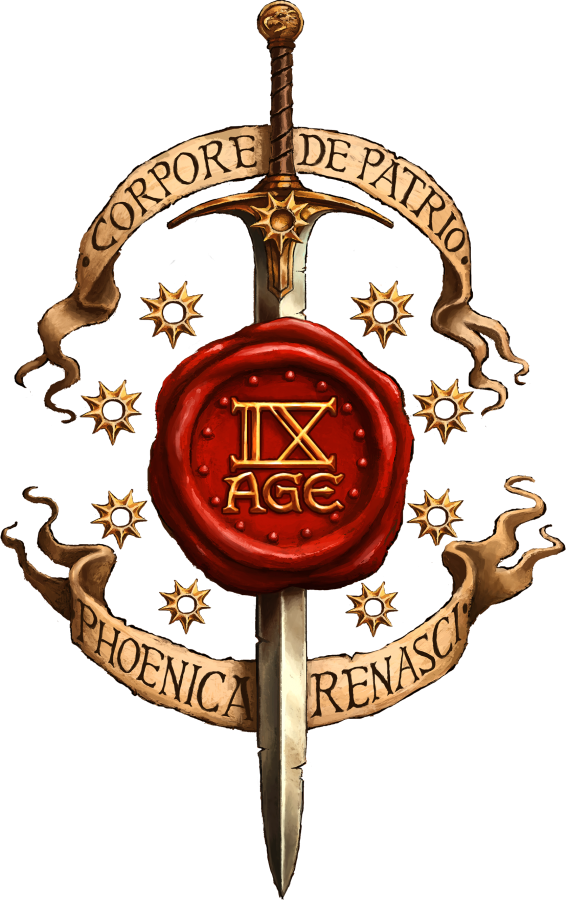
\includegraphics[width=9cm]{../Layout/pics/logo_9th.png}
\vfill
{\antiquefont\fontsize{12}{14.4}\selectfont \textit{\labels@creators}} \\


\end{center}

\newpage

\thispagestyle{empty}

\vphantom{1pt}
\vfill

{\fontsize{12}{14.4}\selectfont

\labels@secondpageannouncement{}

\noindent\newrule{\labels@rulechanges}

\bigskip
\noindent \labels@latexcredit
}


\end{titlepage}

\restoregeometry

\armyspecialrules

\armyspecialruleentry{\mastersoftheundead}

The model chosen as the General of the army is automatically designated as the \newrule{Master} and \textbf{must} exchange one known spell for \necromancysignaturespell, regardless of which Path it uses. At the start of any Player turn in which the army does not have a living \newrule{Master}, you may nominate a single character that uses the Path of Necromancy. If the character passes a Leadership test, the model becomes the new \newrule{Master}. If the test is failed, apply \ashestoashes .

\armyspecialruleentry{\ashestoashes}

At the start of any player turn in which the army does not have a living \newrule{Master} and failed to designate a new one, every unit who possess the \ashestoashes special rule must pass a Leadership test or suffer a number of wounds equal to the value by which they test was failed. These wounds are distributed following the rules for \unstable . Units suffer 1 less Wound than they normally would due to the \unstable and \ashestoashes special rules if within the range of the Battle Standard Bearer's \holdyourground . At the end of any phase in which the General is removed as casualty, units with this rule must automatically test for Leadership in the way described above.

\armyspecialruleentry{\newrule{\chillingshriek{X, Y}}}

Part of a model with this special rule may perform a shooting \newrule{special} attack with \range{8}. It can be used after marching and hits automatically. The target suffers X hits with strength equal to Y plus the current number of Wounds of the shooting part of model, where X and Y are the number within the brackets. When rolling to wound, compare the Strength with the target's Leadership instead of Toughness. Wounds caused are \armourpiercing{6} and \magicalattacks . In the combat phase the model may replace its normal attacks to instead scream at one unit that it is in base contact with it.

\armyspecialruleentry{\awaken{X}}

Models with this special rule can \raisewounds of all the units stated within the brackets above their starting size, using any effect with \raisewounds . A unit's starting size is the size they are written as in the army list. Units can be increased even beyond the maximum size written in their unit entry using this rule.

\armyspecialruleentry{\invocation{X}}

Models with this special rule can heal wounds back with \necromancysignaturespell equal to the amount stated in brackets. A unit cannot be increased above its starting size unless affected by a caster with the \awaken{} special rule.

\armyspecialruleentry{\reaper}

\newrule{Units consisting solely of models with this special rule may move through enemy units during the Remaining Moves Sub-Phase. All Models in such units can make a single Close Combat attack against a single unengaged enemy unit which has been moved through. These attacks hit automatically and are distributed towards the unit as a whole.}

\armyspecialruleentry{\vampiric{X}}

Models with this special rule \newrule{have the \fear special rule} and can make march moves as normal even when outside the range of the General's \inspiringpresence . They still have to test Leadership if they are within \distance{8} of enemy units. 

\newrule{At the end of the Close Combat phase, roll a D6 for each unit with this special rule that caused at least one wound during the phase. On the roll of X+ a single wound is Raised to the unit, where X is the number stated within the brackets. Characters must cause wounds and roll for Raised wounds separately from any unit they are joined to.}

\armyspecialruleentry{\wakethedead}

Each time after an Augment spell from Path of \necromancy (including the \necromancyattribute) is resolved against a model with this rule, you may select a single unit within \distance{6} of it. Until the end of the following player turn, all Models in the chosen units have the \lightningreflexes special rule.

\armyspecialruleentry{\necromanticaura}

Units within \distance{6} of one or more models with this special rule suffer 1 less Wound than they normally would due to the \unstable , \ashestoashes special rules. Models with this special rule cannot benefit from the effects of this special rule.


\armynewsection{\bloodlines}

\vampirelords and \vampireheroes may purchase unique upgrades called \bloodpowers , separated in two
categories called \bloodlinepowers and \ancientbloodpowers . Vampires may also be upgraded to become part of a \bloodline , granting them additional bonuses and sometimes restrictions. The \vampirelords and \vampireheroes of an army must either belong to the same \bloodline or none at all.

\armynewsubsection{\bloodline Vampires}

May only purchase powers that are specific to that \bloodline . \bloodlinepowers may be picked by any
Vampire and \ancientbloodpowers may only be taken by \vampirelords . \bloodlinepowers can be duplicated,
\ancientbloodpowers are \oneofakind .

\armynewsubsection{Independent Vampires}

A Vampire that is not part of a \bloodline may choose between non \ancientbloodpowers of all the \bloodlines . All \bloodlinepowers are \oneofakind .

\armynewsubsection{\bloodties{X}}

Certain unit entries in this army book bear the mention \bloodties{}, followed by the name of a \bloodline between brackets. If the \bloodline of the Vampire characters in the army matches the one written within the brackets, you gain access to the upgrade written in this rule on the unit entry.

\separator

\armynewsubsection{\brotherhood \bloodline\dotfill \pts{35/25}}

A \brotherhood Vampire gains +2 Weapon Skill and wears \platearmour . He is restricted to purchasing
only one additional Magic Level and may only use Path of \necromancy . A \brotherhood Vampire cannot
refuse challenges and must issue one whenever possible, unless another Vampire from the same \bloodline does it first.

\bloodties{}: \vampireknights .

\startpricelist

\pricelistitem{Crimson Rage}{65} \textbf{\ancientbloodpower}. For each unsaved wound the Vampire causes in close combat, it immediately makes another close combat attack. These additional attacks cannot confer more attacks.

\pricelistitem{\newrule{Perfect Warrior}}{35} \textbf{\bloodlinepower}. The Vampire has the \weaponmaster
and \lethalstrike special rules. It is equipped with an \ahw , a \halberd , a \gw , a \lance and a \shield.

\pricelistitem{\newrule{Eternal Duellist}}{30} \textbf{\bloodlinepower}. The Vampire may re-roll to hit and to
wound rolls in challenges.

\endpricelist

\separator

\armynewsubsection{\strigoi \bloodline\dotfill \pts{50/40}}

The Vampire's model has +1 Wound, \regeneration{\newrule{5}} and \hatred . The Vampire cannot select any mount except for the \shriekinghorror , may not wear any kind of Armour, can only purchase a single additional Magic Level and must use Path of \wilderness or \necromancy.

\bloodties{}: \ghouls .

\startpricelist

\pricelistitem{\newrule{Ghoul Lord}}{65} \textbf{\ancientbloodpower}. The Vampire gains the special rules \poisonedattacks and \armourpiercing{1}. All \ghouls in the same unit as the Vampire have \hatred and
\armourpiercing{1}.

\pricelistitem{Curse of the Blood}{70} \textbf{\bloodlinepower}. The Vampire gains the special rule
\regeneration{5}. If the Vampire already has \regeneration{} then its save is increased by \newrule{1} point to a maximum of 4+. All \ghouls in the same unit as the Vampire, and any mount ridden by the Vampire, gains the special rules \regeneration{6}. If they already have \regeneration{} then their save is increased by 1 point to a maximum of 4+.

\pricelistitem{\newrule{Bat Form}}{\newrule{65/40}} \textbf{\bloodlinepower}. The Vampire gains the special rules \thunderouscharge and \fly{8}.

\endpricelist

\separator

\armynewsubsection{\vonkarnstein \bloodline\dotfill \pts{25/20}}

The presence of one or more \vonkarnstein Vampires grants +1 Combat Score. Undead units joined by the Vampire may march as if they had the \vampiric{} special rule. The range of \inspiringpresence and \holdyourground of the Vampire is increased by \distance{6}. In addition, the Vampire may re-roll failed \vampiric{} rolls.

\bloodties{}: \darkcoach .

\startpricelist

\pricelistitem{\newrule{Storm Caller}}{50} \textbf{\ancientbloodpower}. All units within \distance{12} of the Vampire gains the \blurry special rule. Once per game the Vampire can grant \lightningattacks and \armourpiercing{2} to itself and all models part of the same unit. This ability is activated at the start of a combat round and lasts until the end of the player turn.

\pricelistitem{Refined Taste}{25} \textbf{\bloodlinepower}. The Vampire has the \vampiric{2} special rule. \newrule{If mounted on a \largetarget it instead has \vampiric{4}}.

\pricelistitem{\newrule{Hour of the Wolf}}{20} \textbf{\bloodlinepower}. The Vampire gains the \awaken{\zombies , \direwolves , \batswarms , \greatbats} special rule. The Vampire gains \swiftstride and confers this special rule to any unit it joins.

\endpricelist

\separator

\armynewsubsection{\lamia \bloodline\dotfill \pts{35/25}}

The Vampire has +2 Ballistic Skill, -1 Attack, \lightningreflexes and \throwingweapons . If the Vampire is not wearing any Armour it also has the \distracting special rule.

\bloodties{}: \courtofthedamned .

\startpricelist

\pricelistitem{Commandment}{50} \textbf{\ancientbloodpower}. All Rank and File models in any unit joined by the Vampire have Weapon Skill 5. If the Vampire is not engaged in combat itself, it can instead choose to grant this bonus to a single friendly unit within \distance{6}.

\pricelistitem{\newrule{Mask of Innocence}}{25} \textbf{\bloodlinepower}. Enemy units in base contact with one or more Vampire with this power have -1 Leadership.

\pricelistitem{\newrule{Mesmerizing Gaze}}{25} \textbf{\bloodlinepower}. Units charging at or fleeing from units containing at least one Vampire with this power roll an additional dice for their charge or flee move and discard the highest.

\endpricelist

\separator

\armynewsubsection{\nosferatu \bloodline\dotfill \pts{\newrule{140/70}}}

The Vampire is a Level 4/2 \wizard , has -1 Attack, -2 Weapon Skill, cannot take any kind of Armour, generates an additional spell and has the \awaken{\zombies , \skeletons} special rule.

A \nosferatu Vampire may generate spells from more than one Path of Magic. Which Paths and how many spells from each Path will be generated has to be stated on the army list.

\bloodties{}: \wraiths .

\startpricelist

\pricelistitem{\newrule{Unbearable Scrutiny}}{50} \textbf{\ancientbloodpower}. At the start of each Magic Phase, the Player may nominate an enemy \wizard within \distance{18} of the Vampire and within Line of Sight. That \wizard cannot add his Magic Level or use \aideddispel against spells cast by this Vampire during this phase.

\pricelistitem{\newrule{Arcane Knowledge}}{25} \textbf{\bloodlinepower}. Non-vortex spells cast by the Vampire gain an additional \distance{3} range. Damage spells instead gain an additional \distance{6}.

\pricelistitem{Forbidden Path}{20} \textbf{\bloodlinepower}. Select a Battle Magic Path other than Path of \nature . The Vampire can generate spells from this Path in addition to those normally available to it.

\endpricelist

\armymagicitems

\armymagicweapons

\startpricelist

\pricelistitem{\newrule{Bow of Nepharet}}{45} This is \boltthrower \artilleryweapon with the following profile: \range{36}, Strength 6, \armourpiercing{1}, \multiplewounds{D3}{}.

\pricelistitem{Blade of Red Thirst}{40} Type: \hw . Can only be taken by Models with the \vampiric{} special rule. \newrule{The Model gains \vampiric{5} if mounted on a \largetarget} and \vampiric{3} otherwise. The Model rolls 1D6 for each \newrule{unsaved} wound inflicted when rolling for wounds Raised by \vampiric{}. Any excess wounds Raised can be used to \raisewounds on the unit that the Model is part of.

\endpricelist

\armymagicarmor

\startpricelist

\pricelistitem{\newrule{Red Plate of Gilles de Raux}}{\newrule{40}} Type : \platearmour . Wearer has +1 Wound.

\endpricelist

\armytalismans

\startpricelist

\pricelistitem{\newrule{Mantle of Night}}{40} \newrule{Models on foot only}. Enemy models in base contact with wearer, and all models allocating close combat attacks at the wearer, do not gain strength bonuses \newrule{of the +X type} conferred by mundane or magical weapons.

\endpricelist

\armyenchanteditems

\startpricelist

\pricelistitem{\newrule{Tullius' Teeth}}{\newrule{50}} \removedrule{Models on foot only}. Wearer and other \rnf models in its unit have the \distracting special rule.

\endpricelist

\armyarcaneitems

\startpricelist

\pricelistitem{Unholy Tome}{35} \boundspell{4}. Contains the spell \necromancyspelltwo from Path of \necromancy .

\pricelistitem{\newrule{Staff of the Vengeful Dead}}{35} \boundspell{3}. If cast successfully this item
casts an Augment, Lasts one turn spell with range \distance{6}. All \undead models in target unit gain +1 Attack.

\pricelistitem{\newrule{Eye of Setesh}}{20} At the end of any Magic Phase, the play may save one unused Magic Dice and add it to the pool of Magic Dice in the next Magic Phase (immediately after rolling Winds of Magic).

\endpricelist

\armymagicbanners

\startpricelist

\pricelistitem{\newrule{Black Standard of Zagvozd}}{75} The unit carrying this banner has \bodyguard{\vampirelord , \vampirehero}. \vampireknights carrying this banner have the \stubborn special rule instead. All models in the unit carrying this banner also have \wardsave{4} against all Ranged Attacks.

\pricelistitem{\newrule{Banner of the Barrows Kings}}{50} \barrowknights , \barrowguards and \barrowkings in this unit have +1 to Hit in close combat.

\endpricelist


\armylist

\lordstitle

%\showunit{
%	name={Comte Vampire},
%	cost={200},
%	profile={Comte Vampire: 6 7 5 5 5 3 7 5 10},
%	type=Infanterie,
%	basesize=20x20,
%	unitsize=1,
%	specialrules={\undead, \fear, \hunger{6}, \awaken{Zombies}, \vampiric},
%	magiclevel=1,
%	magicpaths={\necromancy, \shadows, \death},
%	options={
%		Peut choisir une \bloodline =\unlimited,
%		Peut prendre un unique \bloodpower =\unlimited,
%		Peut prendre des Objets magiques=\upto: 100,
%		\optionschoice{Peut devenir}{
%			\magiclevel{2}=30,
%			\magiclevel{3}=75,
%		},
%		Bouclier=5,
%		\optionschoice{Peut prendre une Armure}{
%			Armure légère=5,
%			Armure lourde=10
%		},
%		\optionschoice{Peut prendre une Arme de corps à corps}{
%			Arme de base additionnelle=5,
%			Hallebarde=10,
%			Lance de cavalerie=10,
%			Arme lourde=15,
%		}
%	},
%	mounts={Monture Squelette=20, Revenant Monstrueux=100, Cortège Flottant \only{\sisterhoodofthesilverkeep}=190, Chauve-Souris Titanesque \only{\strigoi}=200, Dragon Zombie=280}
%}
%
%\showunit{
%	name={Maître Nécromant},
%	cost={150},
%	profile={Maître Nécromant: 4 3 3 3 4 3 3 1 8},
%	type=Infanterie,
%	basesize=20x20,
%	unitsize=1,
%	specialrules={\undead, \awaken{Zombies, Squelettes}},
%	magiclevel=3,
%	magicpaths={\necromancy, \fire, \death},
%	options={
%		Peut prendre des Objets magiques=\upto:100,
%		\magiclevel{4}=60,
%	},
%	mounts={Monture Squelette=20, Revenant Monstrueux=100, Charrette à Cadavres=100}
%}
%
%\heroestitle
%
%
%\showunit {
%	name={Baron Vampire},
%	cost=80,
%	profile={Baron Vampire:   6 6 4 5 4 2 6 4 8},
%	type=Infanterie,
%	basesize=20x20,
%	unitsize=1,
%	specialrules={\undead, \fear, \hunger{6}, \awaken{Zombies}, \vampiric},
%	magicpaths={\necromancy, \shadows, \death},
%	options={
%		Peut choisir une \bloodline =\unlimited,
%		Peut prendre un unique \bloodpower =\unlimited,		
%		Peut prendre des Objets magiques= \upto: 50,
%		Peut être promu Porteur de la Grande Bannière (sauf s'il est \strigoi)=25,
%		\optionschoice{Peut devenir}{
%			\magiclevel{1}=25,
%			\magiclevel{2}=55,
%		},
%		Bouclier=5,
%		\optionschoice{Peut prendre une Armure}{
%			Armure légère=5,
%			Armure lourde=10,
%		},
%		\optionschoice{Peut prendre une Arme de corps à corps}{
%			Arme de base additionnelle=5,
%			Hallebarde=5,
%			Lance de cavalerie=5,
%			Arme lourde=10,
%		}
%	},
%	mounts={Monture Squelette=20, Revenant Monstrueux=120}
%}
%
%\showunit {
%	name={Roi des Tertres},
%	cost=80,
%	profile={Roi des Tertres:   4 4 0 4 5 3 4 3 9},
%	type=Infanterie,
%	basesize=20x20,
%	unitsize=1,
%	specialrules={\multiplewounds{2}{Infanterie, Cavalerie, Bête de Guerre}, \lethalstrike, \undead, \notaleader},
%	equipment={Armure lourde, Bouclier},
%	options={
%		Peut prendre des Objets magiques= \upto: 50,
%		Peut être promu Porteur de la Grande Bannière=25,
%		\optionschoice{Peut prendre une Arme de corps à corps}{
%			Arme de base additionnelle=5,
%			Hallebarde=5,
%			Lance de cavalerie=5,
%			Arme lourde=10,
%		},
%		Peut être amélioré en \unlivingshield=15
%	},
%	mounts={Monture Squelette=25},
%	unitrules={
%		\unitrule{\unlivingshield}{Cette option ne peut être prise que dans une armée où aucun Personnage n'a la règle \vampiric . Les attaques de corps à corps allouées contre un Nécromant ou Maître Nécromant situé au contact socle à socle d'une figurine avec cette règle spéciale doit à la place cibler la figurine avec \unlivingshield , à condition que cette dernière réussisse un test de CC pour chaque attaque (effectuez les jets séparément). Cette capacité ne peut pas être utilisée si le Nécromant, Maître  Nécromant ou la figurine sont engagés l'un ou l'autre dans un défi.}
%	}
%}
%
%\showunit{
%	name={Nécromant},
%	cost={60},
%	profile={Nécromant: 4 3 3 3 3 2 3 1 7},
%	type=Infanterie,
%	basesize=20x20,
%	unitsize=1,
%	specialrules={\undead, \awaken{Zombies, Squelettes}},
%	magiclevel=1,
%	magicpaths={\necromancy, \fire, \death},
%	options={
%		Peut prendre des Objets magiques=\upto:50,
%		\magiclevel{2}=30,
%	},
%	mounts={Monture Squelette=15, Charrette à Cadavres=100}
%}
%
%\showunit {
%	name={Apparition},
%	cost=65,
%	profile={Apparition:   6 3 - 3 3 2 2 3 5,
%		     Âme en Peine: 6 3 - 3 3 2 3 1 5
%	},
%	type=Infanterie,
%	basesize=20x20,
%	unitsize=1,
%	specialrules={\otherworldlyscream{2, 8} \only{Âme en Peine}, \ethereal, \reaper, \undead, \notaleader, \armourpiercing{6} \only{Apparition}, \ashestoashes, \terror},
%	equipment={Arme lourde (Apparition uniquement)},
%	options={
%		\optionschoice{Doit choisir entre}{
%			Apparition=\free,
%			Âme en Peine=30
%		}
%	},
%}
%
%
%\baseunitstitle
%
%\showunit{
%	name={Zombies},
%	cost=60,
%	profile={Zombie: 4 1 0 3 3 1 1 1 2},
%	type=Infanterie,
%	basesize=20x20,
%	unitsize=20,
%	additionalmodels=40,
%	costpermodel=3,
%	specialrules={\invocation{2D6+3}, \undead, \ashestoashes},
%	commandgroup={\commandgroup{musician=10, banner=10}}
%}
%
%\showunit{
%	name={Squelettes},
%	cost=40,
%	profile={Squelette: 4 2 2 3 3 1 2 1 6},
%	type=Infanterie,
%	basesize=20x20,
%	unitsize=10,
%	additionalmodels=50,
%	costpermodel=4,
%	specialrules={\invocation{1D6+3}, \undead, \ashestoashes},
%	equipment={Armure légère},
%	options={
%		Lance=\free,
%		Bouclier=\permodel:1
%	},
%	commandgroup={\commandgroup{champion=10, musician=10, banner=10, bannerallowance=25}}
%}
%
%\showunit{
%	name={Goules},
%	cost=90,
%	profile={Goule: 4 3 - 3 4 1 3 2 6},
%	type=Infanterie,
%	basesize=20x20,
%	unitsize=10,
%	additionalmodels=30,
%	costpermodel=9,
%	specialrules={\poisonedattacks, \invocation{1D6+3}, \undead, \ashestoashes},
%	options={
%		\skirmishers (si l'unité contient 15 figurines ou moins)=\permodel:1,
%		\vanguard \only{\bloodlineunit{\strigois}}=\permodel:2
%	},
%	commandgroup={\commandgroup{champion=10,
%	                            musician=10, bannerrestriction=unités avec \vanguard,
%	                            banner=10, musicianrestriction=unités avec \vanguard}}
%}
%
%\showunit{
%	name={Loups Sinistres},
%	cost=40,
%	profile={
%		Loup Sinistre: 9 3 0 3 3 1 3 1 3},
%	type=Bête de guerre,
%	basesize=25x50,
%	unitsize=5,
%	additionalmodels=10,
%	costpermodel=7,
%	specialrules={\invocation{1D3+3}, \vanguard, \thunderouscharge, \undead, \ashestoashes},
%	commandgroup={\commandgroup{champion=10}}
%}
%
%\showunit{
%	name={Essaims de Chauves-souris},
%	cost=60,
%	profile={
%		Essaim: 1 2 - 2 2 4 3 4 3},
%	type=Nuée,
%	basesize=40x40,
%	unitsize=2,
%	additionalmodels=8,
%	costpermodel=15,
%	specialrules={\invocation{1D6+3}, \disturbingswarm, \undead, \ashestoashes, \fly{6}},
%	unitrules={
%		\unitrule{\disturbingswarm}{Les ennemis au contact d'une ou plusieurs figurines d'Essaim de Chauves-Souris ont -1 en CC (jusqu'à un minimum de 1).}
%	}
%}
%
%\specialunitstitle
%
%
%\showunit{
%	name={Chevaliers des Tertres},
%	cost=120,
%	profile={Chevalier: 4 3 - 4 4 1 3 1 6,
%		Monture Squelette: 8 2 - 3 3 1 2 1 3
%	},
%	type=Cavalerie,
%	basesize=25x50,
%	unitsize=5,
%	additionalmodels=10,
%	costpermodel=24,
%	specialrules={\invocation{2}, \magicalattacks, \multiplewounds{2}{Infanterie, Bête de guerre, Cavalerie}, \lethalstrike \only{Chevaliers}, \ethereal \only{Monture Squelette}, \undead, \ashestoashes},
%	equipment={Armure lourde, Bouclier, Lance de cavalerie, \naturalarmor},
%	commandgroup={\commandgroup{champion=10, musician=10, banner=10, bannerallowance=50}}
%}
%
%\showunit{
%	name={Gardes des Tertres},
%	cost=100,
%	profile={
%		Garde: 4 3 - 4 4 1 3 1 8},
%	type=Infanterie,
%	basesize=20x20,
%	unitsize=10,
%	additionalmodels=30,
%	costpermodel=10,
%	specialrules={\invocation{1D3+3}, \magicalattacks, \multiplewounds{2}{Infanterie, Bête de Guerre, Cavalerie},\lethalstrike, \bodyguard{Général, Roi des Tertres}, \undead, \ashestoashes},
%	equipment={Armure lourde},
%	options={
%		Bouclier=\permodel:1,
%		\optionschoice{Peuvent prendre une Arme de corps à corps}{
%			Hallebarde=\permodel:2,
%			Arme lourde=\permodel:2
%		}
%	},
%	commandgroup={\commandgroup{champion=10, musician=10, banner=10, bannerallowance=50}}
%}
%
%\showunit{
%	name={Goules Monstrueuses},
%	cost=110,
%	profile={Goule Monstrueuse: 6 3 - 4 5 3 2 3 5},
%	type=Infanterie Monstrueuse,
%	basesize=40x40,
%	unitsize=3,
%	additionalmodels=7,
%	costpermodel=48,
%	specialrules={\invocation{2}, \poisonedattacks, \undead, \fear, \ashestoashes,  \regeneration{5}},
%	commandgroup={\commandgroup{champion=10}}
%}
%
%\showunit{
%	name={Monstruosités Vampiriques},
%	cost=126,
%	profile={
%		Monstruosité Vampirique: 6 4 - 5 4 3 4 3 8},
%	type=Infanterie Monstrueuse,
%	basesize=40x40,
%	unitsize=3,
%	additionalmodels=5,
%	costpermodel=42,
%	specialrules={\invocation{2}, \frenzy, \undead, \fear, \hunger{6}, \skirmishers, \vampiric, \fly{9}},
%	commandgroup={\commandgroup{champion=10}}
%}
%
%\showunit{
%	name={Horde de Spectres},
%	cost=70,
%	profile={Horde de Spectres: 6 3 - 3 3 4 1 4 4},
%	type=Infanterie,
%	basesize=40x40,
%	unitsize=2,
%	additionalmodels=4,
%	costpermodel=35,
%	specialrules={\invocation{1D3+3}, \ethereal, \undead, \fear, \ashestoashes}
%}
%
%\showunit{
%	name={Grandes Chauves-Souris},
%	cost=40,
%	profile={
%		Grandes Chauves-Souris: 1 3 - 3 3 2 3 2 3},
%	type=Bête de guerre,
%	basesize=40x40,
%	unitsize=2,
%	additionalmodels=7,
%	costpermodel=14,
%	specialrules={\invocation{1D3+3}, \undead, \ashestoashes, \skirmishers, \fly{10}},
%}
%
%\showunit{
%	name={Vampire Lupiforme},
%	cost=150,
%	profile={
%		Vampire Lupiforme: 8 5 - 6 5 4 4 5 7},
%	type=Bête Monstrueuse,
%	basesize=50x50,
%	unitsize=1,
%	specialrules={\invocation{1}, \hatred, \undead, \fear, \regeneration{4}, \hunger{3}, \vampiric},
%	options={
%		\optionschoice{Peut prendre une amélioration parmi}{
%			\vanguard=20,
%			\stomp{D3+1}=20,
%			\fly{8}=40,
%		}
%	}
%}
%
%\showunit{
%	name={Charrette à Cadavres},
%	cost=80,
%	profile={
%		Charrette à Cadavres: - - - 4 4 4 - - -,
%   		Maître des Cadavres: - 3 - 3 - -  3 1 5,
%		Horde Chancelante: 4 1 - 3 3 -  1 * -	
%	},
%	type=Char,
%	basesize=50x100,
%	unitsize=1,
%	specialrules={\invocation{1}, \randomattacks{2D6}\only{Horde Chancelante}, \supernaturalaura, \cart, \undead, \ashestoashes, \regeneration{4}},
%	equipment={Armure Naturelle},
%	options={
%		\endlesshorde=25,
%		\optionschoice{Peut prendre une amélioration parmi}{
%			\infernalpyre=10,
%			\unholyconvergence=15,
%			\anticrumbleaura=20
%		}
%	},
%	unitrules={
%		\unitrule{\cart}{La Charrette à Cadavres peut effectuer une Marche Forcée même si elle est de type Char, cependant elle perd la règle spéciale \swiftstride .}
%		\unitrule{\endlesshorde}{La Charrette à Cadavres gagne la règle spéciale \warplatform, mais ne peut rejoindre que des Zombies. Le Maître des Cadavres peut alors participer aux défis comme s'il était le champion de l'unité de Zombies rejointe.}
%		\unitrule{\infernalpyre}{Les Sorciers ennemis dans un rayon de \distance{24} d'une ou plusieurs Charrettes à Cadavres avec cette option souffrent d'un malus de -1 à leurs tentatives pour lancer les sorts.}
%		\unitrule{\unholyconvergence}{Les Sorciers amis font récupérer à leurs cibles de taille Petite deux PVs supplémentaires, et un pour les cibles de taille Moyenne, lorsqu'ils lancent le sort Adjuration des Morts dans un rayon de \distance{6} d'une ou plusieurs Charrettes à Cadavres.}
%	}
%}
%	
%\rareunitstitle
%
%
%\showunit{
%	name={Chevaliers Vampires},
%	cost=225,
%	profile={
%		Chevalier: 4 5 3 5 4 2 5 2 8,
%		Palefroi Mort-Vivant: 8 3 0 4 3 1 2 1 3
%	},
%	type=Cavalerie,
%	basesize=25x50,
%	unitsize=5,
%	additionalmodels=5,
%	costpermodel=45,
%	specialrules={\invocation{2}, \undead, \fear, \hunger{6}, \vampiric},
%	equipment={Lance de cavalerie, Armure lourde, Bouclier, Caparaçon},
%	options={
%		Armure de plates et \devastatingcharge \only{\bloodlineunit{\blooddrakes}}=\permodel:15
%	},
%	commandgroup={\commandgroup{champion=10, musician=10, banner=10, bannerallowance=75}}
%}
%
%\showunit{
%	name={Apparitions Vagabondes},
%	cost=150,
%	profile={
%		Apparition Vagabonde: 6 3 - 3 3 2 2 2 5
%	},
%	type=Infanterie,
%	basesize=20x20,
%	unitsize=5,
%	additionalmodels=3,
%	costpermodel=30,
%	specialrules={\invocation{2}, \wizardconclave{Niveau 1, Le baiser de la Faucheuse, Char de l'Ankou}, \ethereal,  \bodyguard{Apparition, Âme en Peine}, \reaper,  \undead, \armourpiercing{6}, \ashestoashes, \terror, \skirmishers},
%	equipment={Arme lourde},
%	commandgroup={\commandgroup{champion=70, championrestriction=\bloodlineunit{\nosferatu}}},
%}
%
%\showunit{
%	name={Moissonneurs Ardents},
%	cost=150,
%	profile={Moissonneur Ardent: 6 3 - 3 3 1 2 1 5,
%	         Monture Squelette: 8 2 - 3 3 1 2 1 3
%	},
%	type=Cavalerie,
%	basesize=25x50,
%	unitsize=5,
%	additionalmodels=5,
%	costpermodel=30,
%	specialrules={\invocation{2}, \flamingattacks \only{Moissonneur Ardent}, \ethereal, \reaper, \undead, \armourpiercing{6} \only{Moissonneur Ardent}, \ashestoashes,  \freereform, \terror},
%	equipment={Arme lourde},
%	commandgroup={\commandgroup{champion=10}}
%}
%
%\newpage
%\showunit{
%	name={Séraphins de la Mort},
%	cost=150,
%	profile={
%        	Séraphin: 6 5 3 5 5 4 4 3 10,
%	},
%	type=Infanterie Monstrueuse,
%	basesize=50x75,
%	unitsize=2,
%	additionalmodels=3,
%	costpermodel=75,
%	specialrules={\invocation{2}, \anticrumbleaura, \undeadconstructs, \lethalstrike, \undead, \ashestoashes, \terror, \fly{6}},
%	equipment={\innatedefence{5}},
%	options={
%			Armure légère=\permodel:10,
%		\optionschoice{Peut prendre une Arme de corps à corps}{
%			Arme de base additionnelle=\permodel:5,
%			Hallebarde=\permodel:10
%		}
%	},
%	unitrules={
%		\unitrule{\undeadconstructs}{Les figurines avec cette règle subissent une blessure de moins lorsqu'elles appliquent les règles \unstable et \ashestoashes .}
%	},
%}
%
%\showunit{
%	name={Machine Nécrotique},
%	cost=200,
%	profile={
%		Machine Nécrotique: -  - - 5 5 5 - - -,
%       	Maître (1): -  3 1 3 - - 3 1 5,
%		Âme en Peine (0-1): -  3 - 3 - [2] 3 3 5,
%		Attelage de Spectres (1): 8 3 - 3 - - 2 * 4
%	},
%	type=Char,
%	basesize=50x100,
%	unitsize=1,
%	specialrules={\invocation{1}, \randomattacks{2D6} \only{Attelage de Spectres}, \necroticaura, \otherworldlyscream{2,8} \only{Âme en Peine},  \ethereal \only{Attelage de Spectres}, \largetarget , \undead , \ashestoashes , \terror , \regeneration{4}},
%	equipment={\innatedefence{5}},
%	options={
%		\optionschoice{Peut prendre une amélioration parmi}{
%			Âme en Peine (1)=20,
%			\infernaltome=20
%		}
%	},
%	unitrules={
%		\unitrule{\infernaltome}{Les Sorciers amis à moins de \distance{12} d'au moins une Machine Nécrotique équipée d'un \infernaltome ajoutent +2 à leurs tentatives de lancement de sorts de la Discipline \necromancy . Tout Sorcier subissant un Fiasco à moins de \distance{12} d'une Machine Nécrotique équipée d'un \infernaltome compte comme ayant utilisé deux dés de pouvoirs supplémentaires pour lancer le sort.}
%		\unitrule{\necroticaura}{Au début de chacun de vos tours, vous pouvez choisir l'un des effets suivants. Dans les deux cas, X est la valeur du tour de jeu actuel.
%			\begin{customsubitemize}
%				\item Toutes les unités à moins de \distance{6+X} gagnent la règle spéciale \regeneration{6} jusqu'à la fin du tour de joueur suivant. Placez un marqueur à côté des unités affectées par la \regeneration{} après avoir déterminé l'aire d'effet. Une unité ayant déjà la règle spéciale \regeneration{} améliore sa sauvegarde de \regeneration{} d'un point pour obtenir 4+ au mieux.
%				\item Toutes les unités ennemies à moins de \distance{12} subissent 1D6 touches de Force X.}
%			\end{customsubitemize}
%	}
%}
%
%\showunit{
%	name={Chauve-Souris Titanesque},
%	cost=200,
%	profile={
%        	Chauve-Souris Titanesque: 6 4 - 5 6 6 2 4 4,
%	},
%	type=Monstre,
%	basesize=100x150,
%	unitsize=1,
%	specialrules={\invocation{1}, \otherworldlyscream{6, 4}, \undead, \ashestoashes, \regeneration{6}, \fly{8}},
%}
%
%\showunit{
%	name={Carrosse Impie},
%	cost=190,
%	profile={
%		Carrosse Impie:             - - - 5 6 4 - - -,
%        Apparition (1):             - 3 - 3 - - 3 3 5,
%		Vampire Éveillé (*):        - 6 - 5 - - 6 4 8,
%		Palefroi Mort-Vivant (2): 8 3 - 4 - - 2 1 -
%	},
%	type=Char,
%	basesize=50x100,
%	unitsize=1,
%	specialrules={\invocation{1}, \evocationofsouls, \scythes, \undead, \wardsave{4}, \hunger{4}, \terror, \vampiric, \hunger{2} \only{Vampire Éveillé}},
%	equipment={Armure lourde, \naturalarmor, Arme lourde (Apparition uniquement)},
%	options={
%		\stubborn \only{\bloodlineunit{\voncastelstein}}=30
%	},
%	unitrules={
%		\unitrule{\evocationofsouls}{Pour connaître les effets de cette règle spéciale, le joueur doit tenir le décompte des blessures infligées par la figurine. À la fin de chaque Phase de Corps à Corps, observez le nombre total de blessures infligées pour déterminer le niveau d'Intensification de Pouvoir qu'obtient la figurine. Le Carrosse Impie accumule toutes les améliorations jusqu'à son niveau actuel d'Intensification de Pouvoir.
%			\begin{customdescription}
%				\item [1-3 Blessures:] L'air est empli de pulsations meurtrières. Le Carrosse Impie gagne \lethalstrike et \multiplewounds{2}{Infanterie, Bête de Guerre, Cavalerie}.
%				\item [4-6 Blessures:] La nuit s'illumine de feux impurs. Le Carrosse Impie gagne \grindingattacks{1D3} ainsi que \flamingattacks .
%				\item [7-9 Blessures:] Un mal ancien se réveille. Le Carrosse Impie ajoute le Vampire Éveillé à son équipage.
%				\item [10-12 Blessures:] Un vent de terreur souffle dans la nuit et des ombres menaçantes percent dans le ciel. Le Carrosse Impie obtient \fly{8}.
%				\item [13+ Blessures:] Terrorisant. Le Carrosse Impie devient \ethereal .
%			\end{customdescription}
%		}
%	}
%}
%
%\showunit{
%	name={Cortège Flottant},
%	cost=190,
%	profile={
%		Cortège:                    - - - 5 5 5 - - -,
%       	Favorite (3):              - 5 5 5 - - 6 2 7,
%		Attelage de Spectres (1): 8 3 - 3 - - 2 * 4
%	},
%	type=Char,
%	basesize=50x100,
%	unitsize=1,
%	specialrules={\invocation{1}, \randomattacks{2D6} \only{Attelage de Spectres}, \ethereal \only{Attelage de Spectres}, \largetarget, \undead, \ashestoashes, \wardsave{4}, \hunger{6}, \terror, \vampiric},
%	equipment={Armes de jet (Favorites uniquement), \innatedefence{5}},
%	options={
%		\supernaturalaura \only{\bloodlineunit{\sisterhoodofthesilverkeep}}=25
%	}
%}
%
%
%\mountstitle
%
%
%Cette section est réservée aux montures de personnages. Les figurines qui n'en sont pas suivent les règles de leurs entrées d'armée respectives. 
%
%\showunit{
%	name={Monture Squelette},
%	cost={-},
%	profile={
%        		Monture: 8 2 0 3 3 1 2 1 3,
%	},
%	type=Cavalerie,
%	basesize=25x50,
%	unitsize=1,
%	specialrules={\ethereal \only{Monture}, \undead},
%	options={
%		\naturalarmor =10,
%		\fly{8}=15
%	}
%}
%
%\showunit{
%	name={Revenant Monstrueux},
%	cost={-},
%	profile={
%		Revenant Monstrueux: 6  4 - 5 5 4 2 4 4,
%	},
%	type=Bête monstrueuse,
%	basesize=50x50,
%	unitsize=1,
%	specialrules={\largetarget, \invocation{1}, \undead, \fear},
%	options={
%		\optionschoice{Peut prendre jusqu'à deux améliorations parmi}{
%			\poisonedattacks=5,
%			\lethalstrike=10,
%			\hunger{5}=15,
%			\randomattacks{D6+2}=30,
%			\fly{8}=40
%		}
%	}
%}
%
%
%\showunit{
%	name={Chauve-Souris Titanesque},
%	cost={-},
%	profile={
%        	Chauve-Souris Titanesque: 6 4 - 5 6 6 2 4 4,
%	},
%	type=Monstre,
%	basesize=100x150,
%	unitsize=1,
%	specialrules={\invocation{1}, \otherworldlyscream{6,4}, \undead, \ashestoashes, \regeneration{6}, \fly{8}},
%}
%
%\showunit{
%	name={Charrette à Cadavres},
%	cost={-},
%	profile={
%		Charrette à Cadavres: - - - 4 4 4 - - -,
%		Horde Chancelante: 4 1 - 3 3 -  1 * -	
%	},
%	type=Char,
%	basesize=50x100,
%	unitsize=1,
%	specialrules={\invocation{1}, \randomattacks{2D6}\only{Horde Chancelante}, \supernaturalaura, \cart, \undead, \ashestoashes, \regeneration{4}},
%	equipment={\naturalarmor},
%	options={
%		\endlesshorde=25,
%		\optionschoice{Peut prendre une amélioration parmi}{
%			\infernalpyre=10,
%			\unholyconvergence=15,
%			\anticrumbleaura=20
%		}
%	},
%	unitrules={
%		\unitrule{\cart}{La Charrette à Cadavres peut effectuer une Marche Forcée même si elle est de type Char, cependant elle perd la règle spéciale \swiftstride .}
%		\unitrule{\endlesshorde}{La Charrette à Cadavres gagne la règle spéciale \warplatform, mais ne peut rejoindre que des Zombies. Le Maître des Cadavres peut alors participer aux défis comme s'il était le champion de l'unité de Zombies rejointe.}
%		\unitrule{\infernalpyre}{Les Sorciers ennemis dans un rayon de \distance{24} d'une ou plusieurs Charrettes à Cadavres avec cette option souffrent d'un malus de -1 à leurs tentatives pour lancer les sorts.}
%		\unitrule{\unholyconvergence}{Les Sorciers amis font récupérer à leurs cibles de taille Petite deux PVs supplémentaires, et un pour les cibles de taille Moyenne, lorsqu'ils lancent le sort Adjuration des Morts dans un rayon de \distance{6} d'une ou plusieurs Charrettes à Cadavres.}
%	}
%}
%
%\showunit{
%	name={Cortège Flottant},
%	cost={-},
%	profile={
%		Cortège: -  - - 5 5 5 - - -,
%        Favorite (2): -  5 5 5 - - 6 2 7,
%		Attelage de Spectres (1): 8 3 - 3 - - 2 * 4
%	},
%	type=Char,
%	basesize=50x100,
%	unitsize=1,
%	specialrules={\invocation{1}, \randomattacks{2D6} \only{Attelage de Spectres}, \ethereal \only{Attelage de Spectres}, \largetarget, \undead, \ashestoashes, \wardsave{4}, \hunger{6}, \terror, \vampiric},
%	equipment={Armes de jet (Favorites uniquement), \innatedefence{5}},
%	options={
%		\supernaturalaura \only{\bloodlineunit{\sisterhoodofthesilverkeep}}=25
%	}
%}
%
%\showunit{
%	name={Dragon Zombie},
%	cost={-},
%	profile={
%		Dragon Zombie: 6  4 - 6 6 6 2 5 4,
%	},
%	type=Monstre,
%	basesize=50x100,
%	unitsize={1},
%	specialrules={\breathweapon{Force 2, \armourpiercing{6}}, \distracting, \invocation{1}, \undead, \ashestoashes, \regeneration{6}, \fly{7}},
%	equipment={\innatedefence{4}},
%	options={
%		Peut être amélioré en \greaterzombiedragon=40
%	},
%	unitrules={
%		\unitrule{\greaterzombiedragon}{La figurine obtient +1 en CC, améliore la valeur de sa \innatedefence{} de 1, et change de socle pour une taille de \unit{100x150}{\milli\meter}.}
%	}
%}

\end{document}